\documentclass[12pt,a4paper]{report}
\usepackage{graphicx}
\usepackage{setspace}
\usepackage[top=2.5cm, bottom=2cm, left=3cm, right=2cm]{geometry}
\usepackage{lmodern}
\usepackage{parskip}
\usepackage{fancyhdr}
\usepackage{xcolor}
\usepackage{fontspec}
\setmainfont{Times New Roman}
\usepackage{biblatex}
\usepackage[colorlinks=true, linkcolor=black, citecolor=blue, urlcolor=blue]{hyperref}
\usepackage{etoolbox}
\usepackage{titlesec}
\addbibresource{references.bib}
\usepackage{booktabs}
\usepackage{tabularx}
\usepackage{float}
\usepackage{amsmath, amssymb, amsthm}
\usepackage{tocloft}
\usepackage{enumitem}
\usepackage{caption}
\usepackage{subcaption}
\usepackage{array}
\usepackage{longtable}
\usepackage{multirow}
\usepackage{algorithm}
\usepackage{algpseudocode}
\usepackage{listings}
\usepackage{pifont}
\usepackage{microtype}
\emergencystretch=3em
\hyphenation{Sim-pli-cial-LDLT Per-Ver-tex-Norm-al-ized-Per-Face Per-Face-Norm-al-ized}
\usepackage{tikz}
\usepackage{pgfplots}
\pgfplotsset{compat=1.18}
\usetikzlibrary{arrows.meta, positioning, calc, shapes.geometric,
                decorations.pathmorphing, decorations.markings,
                patterns, fit, backgrounds, 3d, shadings}

% Reduce heading leading skip
\setlength{\cftbeforetoctitleskip}{0cm}
\setlength{\cftbeforeloftitleskip}{0cm}
\setlength{\cftbeforelottitleskip}{0cm}

\titlespacing*{\chapter}{0pt}{0cm}{1cm}

\definecolor{ackblue}{HTML}{365f91}
\DefineBibliographyStrings{english}{%
  bibliography = {REFERENCES},
}

\makeatletter
\renewcommand{\listfigurename}{\textcolor{ackblue}{\Large \textbf{LIST OF FIGURES}}}
\renewcommand{\listtablename}{\textcolor{ackblue}{\Large \textbf{LIST OF TABLES}}}
\renewcommand{\contentsname}{\textcolor{ackblue}{\Large \textbf{TABLE OF CONTENTS}}}
\makeatother

\newcommand{\CustomChapter}[1]{%
  \clearpage
  \vspace*{0cm}
  \begin{center}
    \textcolor{ackblue}{\Large \textbf{#1}}
  \end{center}
  \vspace{1cm}
}

% Listings style for C++ code snippets
\lstdefinestyle{cppstyle}{
    basicstyle=\ttfamily\footnotesize,
    keywordstyle=\color{blue}\bfseries,
    commentstyle=\color{gray}\itshape,
    stringstyle=\color{red!60!black},
    numbers=left,
    numberstyle=\tiny\color{gray},
    stepnumber=1,
    numbersep=6pt,
    showstringspaces=false,
    breaklines=true,
    frame=single,
    rulecolor=\color{black!30},
    tabsize=2,
    language=C++
}
\lstset{style=cppstyle}

\pagestyle{plain}

\begin{document}
\onehalfspacing

% ---------------- Page 1 (Cover) ----------------
\begin{titlepage}
    \thispagestyle{empty}
    \centering
    \textbf{VIETNAM NATIONAL UNIVERSITY OF HOCHIMINH CITY} \\
    \textbf{THE INTERNATIONAL UNIVERSITY} \\
    \textbf{SCHOOL OF COMPUTER SCIENCE AND ENGINEERING} \\
    \vspace{1cm}

    
\includegraphics[width=0.3\textwidth]{images/logo-vector-IU-01.png} \\

    \vspace{1cm}
    \Large
    \textbf{NORMAL FIELD DIFFUSION FOR GEOMETRY-AWARE HOLE FILLING IN 3D TRIANGLE MESHES:\\ A MESHLAB PLUGIN IMPLEMENTATION} \\
    \vspace{0.5cm}
    \vspace{1.5cm}

    \normalsize
    By \\
    \textbf{Truong Tri Dung} \\
    \textbf{MITIU25208} \\

    \vfill

    \begin{singlespace}
    A project report submitted to the School of Computer Science and Engineering \\
    in partial fulfillment of the requirements for the course \\
    Advanced Computer Graphics
    \end{singlespace}

    \vspace{1cm}
    \textbf{Ho Chi Minh City, Vietnam} \\
    Year 2026 \\

\end{titlepage}

\newpage
\pagenumbering{arabic}
\setcounter{page}{2}

% ---------------- TABLE OF CONTENTS ----------------
\newpage
\phantomsection
\addcontentsline{toc}{chapter}{TABLE OF CONTENTS}
\begingroup
\let\addcontentsline\relax
\tableofcontents
\endgroup

% ---------------- LIST OF FIGURES ----------------
\newpage
\phantomsection
\addcontentsline{toc}{chapter}{LIST OF FIGURES}
\listoffigures

% ---------------- LIST OF TABLES ----------------
\newpage
\phantomsection
\addcontentsline{toc}{chapter}{LIST OF TABLES}
\listoftables

% ---------------- ABSTRACT ----------------
\newpage
\CustomChapter{ABSTRACT}
\addcontentsline{toc}{chapter}{ABSTRACT}

Triangle meshes from scan or reconstruction pipelines often contain holes, and most existing fillers produce visibly flat patches because they triangulate the boundary in a plane. This report describes a MeshLab plugin implementing \emph{Normal Field Diffusion} (NFD), which gives the patch its curvature in two stages. The boundary vertex normals are treated as Dirichlet data and diffused across the patch interior using the heat equation. Each interior vertex is then displaced along its diffused normal by an amount derived from a spherical-cap fit to the boundary. Implicit Euler with a one-time Cholesky factorisation keeps the inner solver stable and inexpensive. On six ground-truth meshes (spheres, cylinder, torus, Stanford Bunny, cow), the symmetric Hausdorff error reaches 0.12\% on the simplest case and is roughly $2$--$4\times$ smaller than MeshLab's built-in \texttt{Close Holes} filter on curved surfaces.

\vspace{0.4cm}
\noindent\textbf{Keywords:} hole filling, mesh repair, cotangent Laplacian, heat equation, MeshLab.

%
\definecolor{ackblue}{HTML}{365f91}
\titleformat{\chapter}[display]
  {\normalfont\bfseries\color{ackblue}\filcenter}
  {\Large\MakeUppercase{Chapter \thechapter}}{0pt}
  {\Large\MakeUppercase}
\titleformat{\section}
  {\color{ackblue}\bfseries}
  {\thesection.}{0.5em}{}
\titleformat{\subsection}
  {\color{ackblue}\bfseries}
  {\thesubsection.}{0.5em}{}

\chapter{INTRODUCTION}

\section{Background}

Mesh data from scanners or photogrammetry is rarely watertight. Self-occlusion, low-confidence regions, glossy surfaces, and post-process editing all introduce holes. The presence of a hole is enough to break rendering (the back side becomes visible through it), most physical simulations (which assume a closed domain), and 3D-print slicers.

Standard hole fillers, such as ear clipping or the advancing-front method behind MeshLab's \texttt{Close Holes}, close the topological gap but produce a patch that is essentially flat. On a sphere this is immediately visible as a dimple. More sophisticated alternatives exist --- Poisson reconstruction, thin-plate splines --- but they either reshape the entire mesh or require solving a fourth-order PDE, neither of which fits an interactive plugin model.

The hole-filling problem appeared on the Advanced Computer Graphics project list, but only the problem itself was specified, not the approach. NFD was chosen after a short literature survey: the Verdera et al.\ paper on inpainting surface holes offered the most direct route from boundary normals to a curved patch, and most of its machinery (cotangent Laplacian, heat equation, sparse linear solvers) was already covered in the course.

\begin{figure}[H]
    \centering
    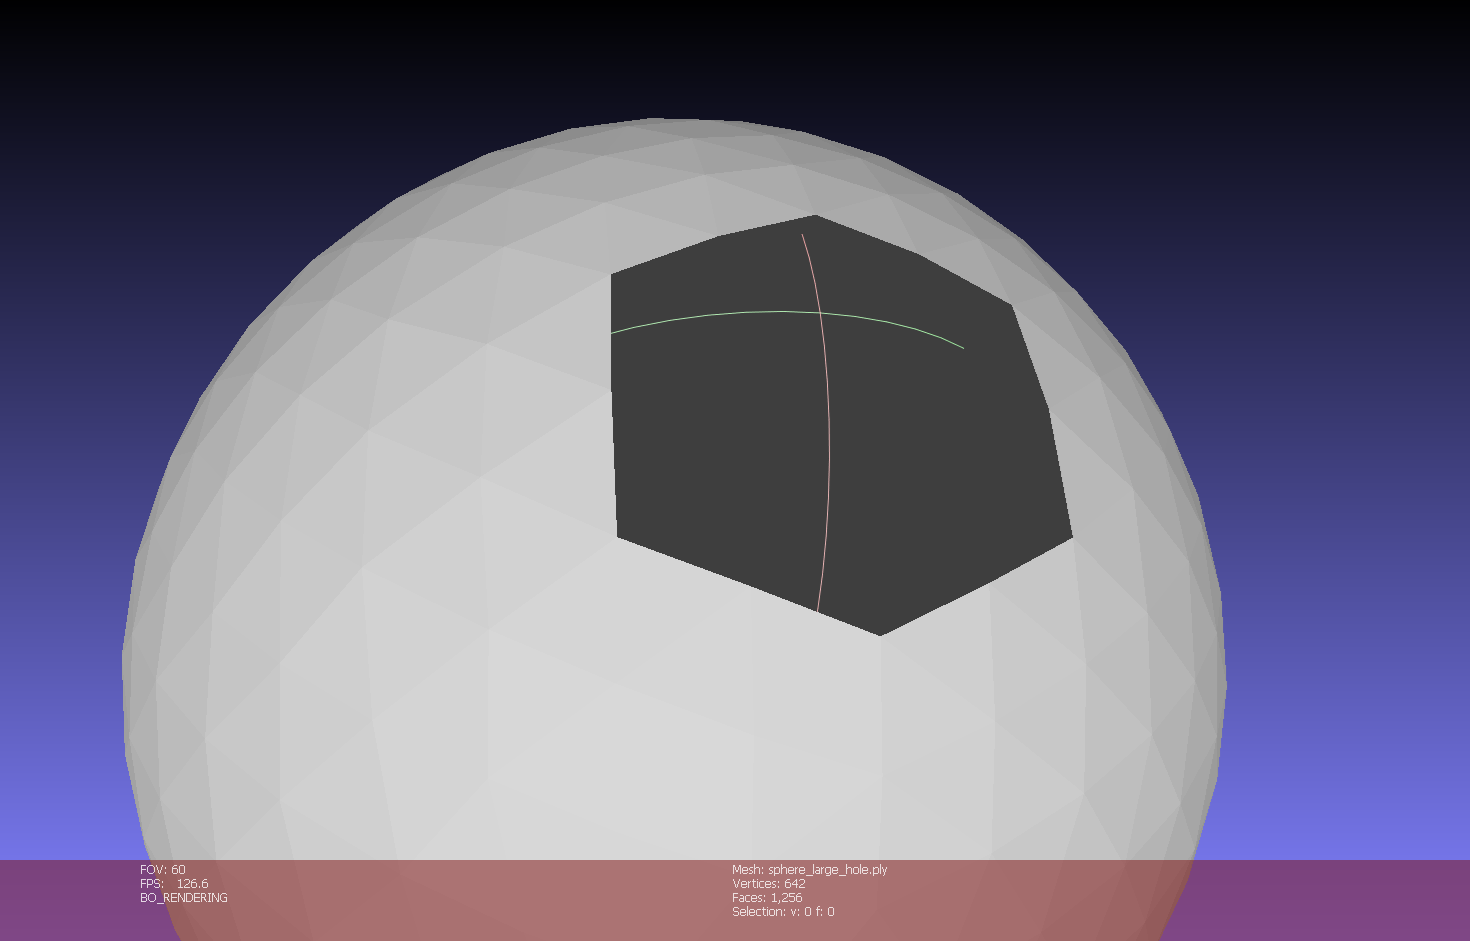
\includegraphics[width=0.45\textwidth]{figures/fig_teaser_hole.png}
    \hfill
    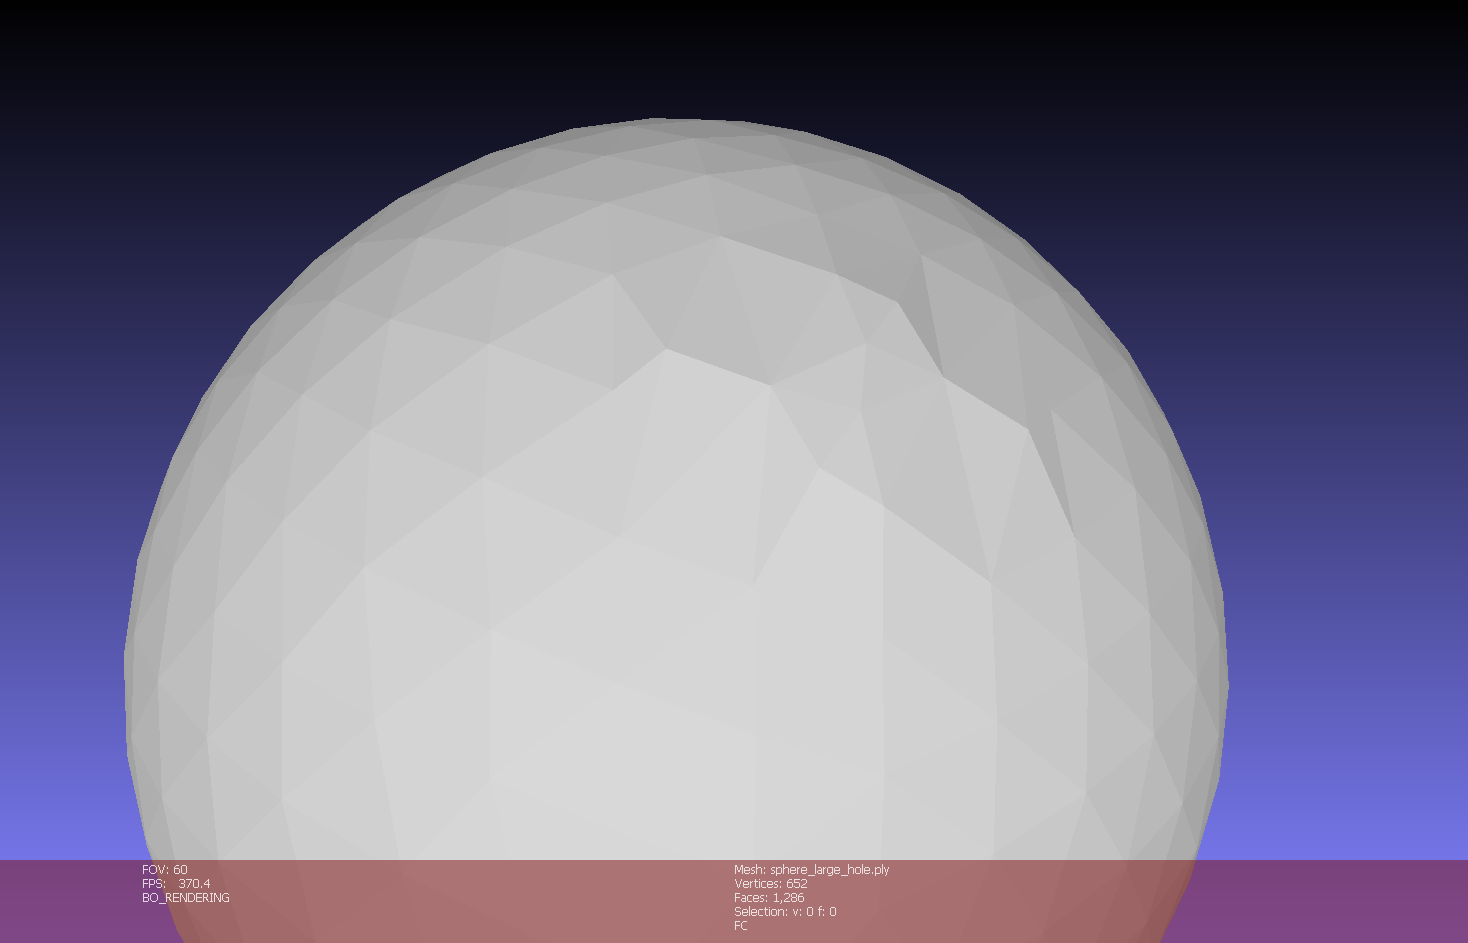
\includegraphics[width=0.45\textwidth]{figures/fig_teaser_filled.png}
    \caption{Input mesh with a hole (left) and the NFD result (right).}
    \label{fig:teaser}
\end{figure}

Normal Field Diffusion (NFD) sits between these extremes. It triangulates the hole as a flat patch first, then diffuses the boundary normals across the patch interior using a discrete heat equation, and finally displaces each interior vertex along its diffused normal by an amount estimated from the boundary geometry. The patch ends up curved, matches the surrounding surface, and the rest of the mesh is left alone.

\section{Problem and scope}

Given a mesh $\mathcal{M} = (V, F)$ with one or more boundary loops, the goal is to add vertices and faces so that each loop becomes interior, the patch joins the surrounding surface continuously, and the new triangles are roughly the same size and shape as their neighbours. The topological closure is trivial. Triangle quality is handled by standard heuristics. The hard part is geometric continuity, which is what this report focuses on.

The implementation is a self-contained MeshLab plugin in C++ on top of VCGlib and Eigen. It processes one hole at a time, leaves everything else untouched, and exposes seven parameters in the standard filter dialog. Evaluation uses MeshLab's built-in Hausdorff sampler against ground-truth meshes generated from the same source models.

\section{Outline}

Chapter~2 surveys related work and places NFD in context. Chapter~3 collects the mathematical background --- discrete Laplace--Beltrami, the heat equation, implicit Euler, Taubin smoothing. Chapter~4 walks through the seven pipeline stages. Chapter~5 covers the plugin implementation. Chapter~6 reports the Hausdorff measurements and compares NFD with MeshLab's \texttt{Close Holes} filter. Chapters~7 and~8 discuss limitations and conclude.

\chapter{RELATED WORK}

Hole filling on triangle meshes has a long history. The papers that turned out to matter for this project fall into three rough groups: combinatorial methods that triangulate the hole as a polygon, variational methods that solve a global energy on the patch, and normal-field methods that propagate orientation information from the boundary inward. NFD borrows from all three and is closest in spirit to the third.

\section{Combinatorial fillers}

The ear-clipping family is the oldest. Meisters~\cite{meisters1975} proved in 1975 that every simple polygon has at least two ears, which is the topological fact that makes ear clipping work. Held's FIST system~\cite{held2001} is the robust industrial implementation, and most mesh-tool ear clippers descend from it either directly or by reimplementation. The version in this report borrows the layered fallback structure from FIST without using its exact-arithmetic predicates, because the patch sizes encountered here are small enough that ordinary floating-point comparisons do not cause trouble.

For 3D hole filling the canonical reference is Liepa~\cite{liepa2003}, an advancing-front method that picks each new triangle directly in 3D rather than projecting to 2D and lifting back. Liepa is what MeshLab's \texttt{Close Holes} filter implements, and it is the direct baseline this report compares against in Chapter~6. The patch it produces is geometrically flat in the following sense: each new triangle is chosen on local quality criteria (dihedral angle, edge length, balance of the front) without any input from the curvature of the surrounding mesh. On a sphere this is immediately visible.

Barequet and Sharir~\cite{barequet1995} formulate the same problem as a constrained Delaunay triangulation, which is theoretically cleaner but expensive and not native to the MeshLab/VCGlib tooling. The standard approximation is Lawson-flip iteration, which locally improves quality without solving the global problem. The implementation here applies it twice, once after initial ear clipping and once after centroid refinement.

The combinatorial line shares one structural limit. The patch is fully determined by the boundary polygon and the heuristic, so it cannot reflect curvature information from outside the polygon --- there is no mechanism for that to enter. The next two groups of work address this in different ways.

\section{Variational and PDE methods}

The simplest variational approach treats the patch as a discrete minimum surface and solves $\Delta u = 0$ on patch positions with the boundary fixed. It is fast, gives a smooth patch, and biases toward flatness because it minimises area. On a sphere the patch sits inside the chord rather than on the sphere; the dimple problem of ear clipping is reproduced through different machinery. Botsch and Kobbelt's Laplacian deformation framework~\cite{botsch2004}, although the paper itself is about interactive editing rather than hole filling, is built on the same Laplacian-with-Dirichlet machinery and shares the same shrinkage tendency when adapted to hole filling.

Going to a fourth-order energy --- bi-Laplacian, equivalent to thin-plate splines --- lets the patch encode boundary tangents in addition to positions, and produces $C^2$ patches that can bulge outward when the surrounding surface is curved. Nealen et al.~\cite{nealen2006} present a unified Laplacian/bi-Laplacian framework that covers this as one of several modes. The cost is a denser, worse-conditioned linear system: the bandwidth of $\Delta^2$ is roughly the square of $\Delta$ on a triangle mesh, and direct solvers slow down accordingly. For a plugin that runs inside MeshLab's interactive loop this lives on the wrong side of the speed/quality trade-off.

Of all the references in this section, the closest in spirit to NFD is Pernot, Moraru, and V{\'e}ron~\cite{pernot2006}. Instead of minimising a quadratic energy on positions, they minimise the variation of curvature across the patch, simulated as a thin-plate mechanical model whose boundary forces are driven by the surrounding curvature. The high-level intuition --- carry curvature information from the boundary inward --- is the same as NFD's, but the formulation is on positions, the iteration is non-linear, and the input must be smoothly parameterisable. Reading their paper alongside Verdera et al.\ helped clarify what is actually being asked of the patch: not just a smooth surface, but one whose curvature continues that of the boundary.

Poisson surface reconstruction~\cite{kazhdan2006, kazhdan2013} occupies a different niche. It is not strictly a hole filler --- the input is a point cloud or oriented mesh and the output is a globally smooth surface, with holes filled as a side effect. For hole-repair purposes the difficulty is exactly that. Parts of the input that did not need fixing get reshaped along with the broken parts, and the input-output triangle correspondence is lost in the volumetric intermediate.

Laplacian Surface Editing by Sorkine et al.~\cite{sorkine2004} is mentioned here because of a useful conceptual distinction it sharpens: the Laplacian can be used as an \emph{operator} on positions or as a \emph{representation} of geometry through differential coordinates. Minimum-surface and bi-Laplacian hole fillers use the Laplacian as an operator. Differential-coordinates methods use it as a representation. NFD belongs to the first camp, although its operator is applied to normals rather than positions.

\section{Normal-field and curvature-based methods}

Verdera, Caselles, Bertalm{\'i}o, and Sapiro~\cite{verdera2003} is the closest precursor and where the core idea of NFD originates. They diffuse each component of the surface normal field across the hole through a non-linear PDE, with boundary normals as Dirichlet data, and reconstruct positions afterwards. NFD is essentially this idea translated from level-set surfaces (where they discretise the PDE on a regular volumetric grid) to triangle meshes (where the cotangent Laplacian gives the right discrete operator directly). The level-set framework was a reasonable choice in 2003 because the triangle-mesh discrete-differential-geometry tooling was still settling: Pinkall--Polthier was known but Meyer et al.\ had only just appeared, and not every implementation used cotangent weights as a default. Translating to triangle meshes today is more or less mechanical.

The diffusion idea itself comes from earlier work on image inpainting by Bertalm{\'i}o, Sapiro, Caselles, and Ballester~\cite{bertalmio2000}, from the same research group. Verdera et al.\ is the surface-normals analogue of Bertalm{\'i}o et al.'s pixel-intensities approach. Knowing this connection was useful while reading the surface-holes paper, because the level-set notation is dense and the underlying intuition is clearer when read alongside the 2D image case.

Local normal-interpolation methods are a parallel branch that interpolates boundary normals into the interior without a global PDE. Wang and Oliveira~\cite{wang2007} use radial basis functions, Jun~\cite{jun2005} uses a moving-least-squares approach with sub-region partitioning. Without a global smoothness criterion these methods are simpler to implement but degrade on larger or non-convex holes; the seams between sub-regions in Jun's piecewise approach in particular tend to need separate cleanup.

Zhao, Gao, and Lin~\cite{zhao2007} sit between Verdera et al.\ and the local methods. They use a Poisson-style PDE for fairing patch positions, combined with a separate boundary-driven displacement step. The two-stage structure is the same as Stages~4 and~6 in this report, but the variable they solve for is position, not normal, so the formulation inherits the shrinkage of position-based methods --- partially compensated by the displacement step but not eliminated.

\section{Foundations}

The discrete operators NFD relies on come from the broader discrete-differential-geometry literature. The cotangent Laplacian was introduced by Pinkall and Polthier~\cite{pinkall1993} in 1993 for discrete minimal-surface construction, and was packaged as a standard geometry-processing operator by Meyer et al.~\cite{meyer2003} a decade later, with the mean-curvature normal identity that Stage~2 of NFD uses. Wardetzky et al.~\cite{wardetzky2007discrete} gave the useful negative result that no discrete Laplacian satisfies all desirable properties simultaneously, which retroactively explains why several different cotangent-style operators coexist in the literature. The version used here is convergent and intrinsic but breaks the maximum principle on obtuse triangles, and NFD handles this by clamping negative weights to zero. Sharp and Crane~\cite{sharp2020} address the same problem more cleanly through intrinsic Delaunay remeshing; that would be a worthwhile upgrade for inputs with many obtuse triangles.

Two other operators are reused as-is. Desbrun et al.~\cite{desbrun1999} introduced implicit fairing by diffusion in 1999, which is essentially the numerical recipe NFD uses in Stage~4 (assemble the cotangent Laplacian, solve the implicit-Euler system, iterate) but applied to vertex positions rather than normals. Taubin's $(\lambda, \mu)$ filter~\cite{taubin1995} is the standard non-shrinking low-pass smoother, used in Stage~6 of NFD because uniform Laplacian smoothing would flatten the dome. Crane et al.~\cite{crane2013heat} proposed the heat method for geodesic distance computation, which would be a more accurate replacement for the multi-source Dijkstra in Stage~6; we have not measured how much accuracy it would buy in practice on the test patches.

The mesh-repair survey of Attene, Campen, and Kobbelt~\cite{attene2013} is the right reference for context. Hole filling is one of many mesh-defect classes; a production-grade repair tool needs to handle the others (non-manifold edges, self-intersections, inverted normals) as well. NFD assumes the input has been cleaned of those defects, which is reasonable inside MeshLab where standard cleanup filters are one menu away.

\section{Where NFD sits}

The components of NFD are individually well-known: heat-equation diffusion of normals is from Verdera et al., the cotangent Laplacian is standard, Taubin smoothing dates from 1995. What this report contributes is putting them together in a way that runs end-to-end inside MeshLab without voxelisation, with an implicit-Euler solver and a one-time $LDL^T$ factorisation that keeps the inner loop fast, a spherical-cap displacement model whose dome height is derived from boundary geometry rather than supplied as a parameter, and a $\sqrt{2t-t^2}$ profile that gives tangent-plane continuity at the patch boundary --- the property the more common parabolic profile fails to provide.

Among the closest references --- Verdera et al., Pernot et al., Zhao et al.\ --- none combine these specific choices in the same way. The result is best understood as a practical translation of Verdera-style normal diffusion into the triangle-mesh setting, picked apart into a sequence of stages that each have a clear role and a known fallback when they fail.

\chapter{MATHEMATICAL PRELIMINARIES}

This chapter collects the four pieces of background needed to read Chapter~4: the cotangent Laplacian, the heat equation on a manifold, implicit Euler time stepping, and Taubin smoothing.

\section{Cotangent Laplacian}

A triangle mesh is a pair $\mathcal{M} = (V, F)$ with vertex set $V \subset \mathbb{R}^3$ and triangular face set $F$. An edge is a \emph{border} edge if it belongs to exactly one face; a closed chain of border edges is a hole.

The Laplace--Beltrami operator $\Delta_{\mathcal{S}}$ on a smooth surface admits several discrete versions. The simplest is the uniform Laplacian, $L_u(v_i) = \sum_j (v_j - v_i) / d_i$, which is cheap but mesh-density dependent. The cotangent Laplacian~\cite{pinkall1993, meyer2003} weights each neighbour by
\begin{equation}
w_{ij} = \cot \alpha_{ij} + \cot \beta_{ij}, \label{eq:cot}
\end{equation}
where $\alpha_{ij}$ and $\beta_{ij}$ are the two angles opposite the edge $(v_i, v_j)$ in the two faces sharing it (Figure~\ref{fig:cotangent-weights}). The cotangent Laplacian converges to $\Delta_{\mathcal{S}}$ under refinement, is invariant under intrinsic remeshing, and gives the standard mean-curvature normal $L_{\text{cot}}(v_i) = -2 H_i \mathbf{n}_i$. We use it everywhere in this report.

\begin{figure}[H]
    \centering
    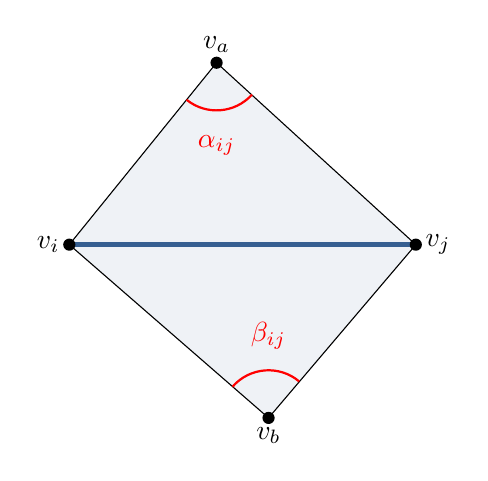
\begin{tikzpicture}[scale=1.1, line join=round]
        \coordinate (vi) at (0, 0);
        \coordinate (vj) at (4, 0);
        \coordinate (va) at (1.7, 2.1);
        \coordinate (vb) at (2.3, -2.0);
        \fill[ackblue!8] (vi) -- (vj) -- (va) -- cycle;
        \fill[ackblue!8] (vi) -- (vj) -- (vb) -- cycle;
        \draw[thick] (vi) -- (vj);
        \draw (vi) -- (va) -- (vj);
        \draw (vi) -- (vb) -- (vj);
        \draw[ultra thick, ackblue] (vi) -- (vj);
        \draw[red, thick] (va) ++(-129:0.55) arc[start angle=-129, end angle=-42, radius=0.55];
        \draw[red, thick] (vb) ++(50:0.55) arc[start angle=50, end angle=139, radius=0.55];
        \fill (vi) circle (2pt); \node[left]  at (vi) {$v_i$};
        \fill (vj) circle (2pt); \node[right] at (vj) {$v_j$};
        \fill (va) circle (2pt); \node[above] at (va) {$v_a$};
        \fill (vb) circle (2pt); \node[below] at (vb) {$v_b$};
        \node[red] at ($(va)+(0, -0.95)$) {$\alpha_{ij}$};
        \node[red] at ($(vb)+(0,  0.95)$) {$\beta_{ij}$};
    \end{tikzpicture}
    \caption{Cotangent weight on edge $(v_i, v_j)$, using the two opposite angles $\alpha_{ij}$ and $\beta_{ij}$.}
    \label{fig:cotangent-weights}
\end{figure}

A practical detail: $\cot \theta < 0$ for obtuse angles, which can break the maximum principle of the discrete Laplacian. We clamp $w_{ij} \leftarrow \max(w_{ij}, 0)$, which is simple and works on the test meshes. The cleaner alternative is intrinsic Delaunay remeshing~\cite{sharp2020}, but that is substantially more code.

\section{Heat equation and implicit Euler}

The heat equation on a domain $\Omega$ with Dirichlet boundary data $g$ is
\begin{equation}
\frac{\partial u}{\partial t} = \lambda \Delta_\Omega u, \qquad u\big|_{\partial\Omega} = g.
\end{equation}
As $t \to \infty$, the solution converges to the harmonic extension of $g$ into $\Omega$ --- the smoothest interpolation in the sense of Dirichlet energy. This is the property we want for the diffused normal field on the patch.

For time stepping there is a choice between explicit and implicit Euler. Explicit Euler is conditionally stable, requiring $\Delta t < 2/\rho(L)$, which gets unfavourable as the mesh refines. Implicit Euler,
\begin{equation}
(I + \lambda L)\, u^{t+1} = u^t, \label{eq:implicit-euler}
\end{equation}
is unconditionally stable for any $\lambda > 0$ when $L$ is positive semi-definite. The matrix $I + \lambda L$ is symmetric positive definite, sparse, and stays the same across iterations --- only the right-hand side changes. This is exactly the case where a one-time Cholesky factorisation pays off.

We use \texttt{Eigen::SimplicialLDLT}, which factors the matrix as $A = LDL^T$ once and then solves each iteration in $O(\text{nnz}(A))$. For the patch sizes we encounter (interior vertex counts of order $10^2$--$10^3$), a single factorisation amortised over 50 iterations is essentially free.

\section{Taubin smoothing}

Plain Laplacian smoothing $v \leftarrow v + \lambda L(v)$ moves each vertex toward the centroid of its neighbours and works well for cleaning high-frequency noise --- but iterated, it shrinks the surface globally. Taubin~\cite{taubin1995} fixes this with a two-step pass: a positive shrink step ($\lambda > 0$) followed by a negative inflate step ($\mu < 0$, $|\mu| > \lambda$). The combined transfer function in the Laplacian eigenbasis,
\begin{equation}
f(k) = (1 - \lambda k)(1 - \mu k),
\end{equation}
satisfies $f(0) = 1$ (DC preserved) and $|f(k)| < 1$ for high frequencies (noise attenuated). The result is a low-pass filter without shrinkage. We use $\lambda = 0.40$, $\mu = -0.44$, three pairs --- a standard choice from the literature.

\chapter{METHODOLOGY}

\section{Pipeline overview}

The plugin runs seven stages per detected hole. Stage~4 is the algorithmic core; the others prepare the patch for it or clean up after it. Stages~5 and~6 must run in this order: uniform Laplacian smoothing applied after displacement would erase the dome that displacement creates, because uniform smoothing exhibits shrinkage on curved surfaces.

This ordering was reversed in an early version of the implementation. Stage~6 produced patches with localised spike artifacts, and applying Stage~5 afterwards seemed like a natural cleanup pass --- right up until the result on \texttt{sphere\_large} was overlaid on the ground truth and the dome turned out to have been quietly flattened. Reordering the two stages and using Taubin (which preserves low frequencies) in Stage~6 for spike cleanup fixed both problems at once.

\begin{figure}[H]
    \centering
    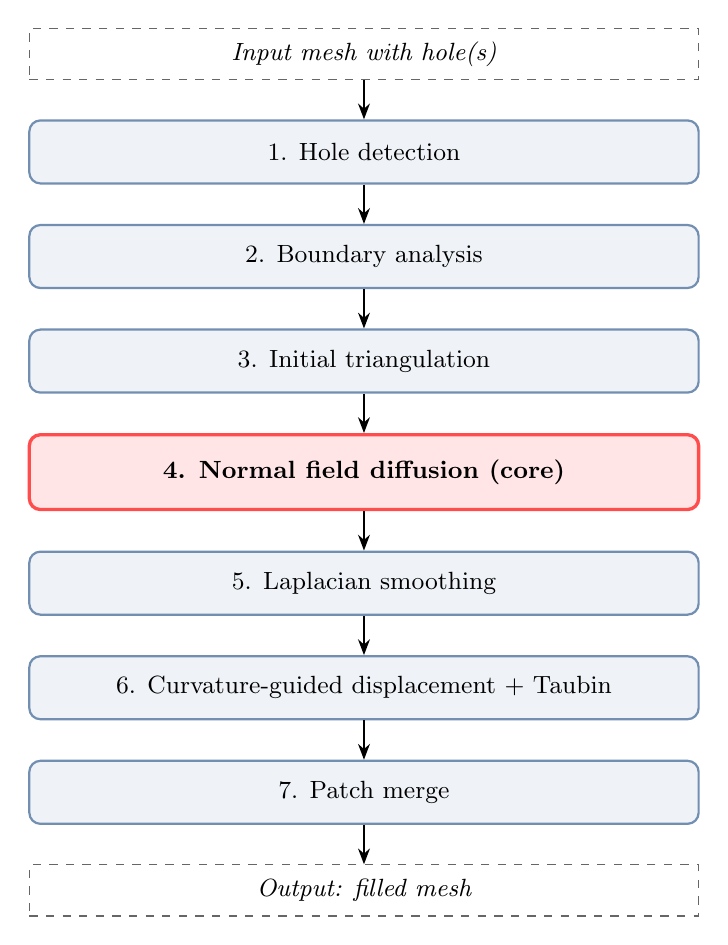
\begin{tikzpicture}[
        node distance=0.5cm,
        stage/.style={rectangle, rounded corners=4pt, draw=ackblue!70, thick,
                      fill=ackblue!8, minimum width=8.5cm, minimum height=0.8cm,
                      align=center, font=\small},
        core/.style={rectangle, rounded corners=4pt, draw=red!70, very thick,
                     fill=red!10, minimum width=8.5cm, minimum height=0.95cm,
                     align=center, font=\small\bfseries},
        io/.style={rectangle, draw=black!60, dashed,
                   minimum width=8.5cm, minimum height=0.65cm, align=center,
                   font=\small\itshape},
        arrow/.style={-{Stealth[length=2mm]}, thick}
    ]
        \node[io] (in) {Input mesh with hole(s)};
        \node[stage, below=of in] (s1) {1. Hole detection};
        \node[stage, below=of s1] (s2) {2. Boundary analysis};
        \node[stage, below=of s2] (s3) {3. Initial triangulation};
        \node[core,  below=of s3] (s4) {4. Normal field diffusion (core)};
        \node[stage, below=of s4] (s5) {5. Laplacian smoothing};
        \node[stage, below=of s5] (s6) {6. Curvature-guided displacement + Taubin};
        \node[stage, below=of s6] (s7) {7. Patch merge};
        \node[io,    below=of s7] (out) {Output: filled mesh};
        \draw[arrow] (in) -- (s1);
        \draw[arrow] (s1) -- (s2);
        \draw[arrow] (s2) -- (s3);
        \draw[arrow] (s3) -- (s4);
        \draw[arrow] (s4) -- (s5);
        \draw[arrow] (s5) -- (s6);
        \draw[arrow] (s6) -- (s7);
        \draw[arrow] (s7) -- (out);
    \end{tikzpicture}
    \caption{The seven-stage pipeline.}
    \label{fig:pipeline}
\end{figure}

\section{Hole detection}

VCGlib's adjacency machinery does most of the work. After enabling face--face and vertex--face adjacency and calling \texttt{UpdateFlags::FaceBorderFromFF}, each border edge has its flag set, and we walk the boundary by hopping from one border edge to the next using \texttt{VFIterator}. In a 2-manifold mesh each boundary vertex has exactly two incident border edges, so excluding the previous vertex uniquely determines the next one.

\begin{algorithm}[H]
\caption{Boundary loop walk}
\begin{algorithmic}[1]
\For{each face $f$, each local edge $e$}
    \If{$\texttt{IsBorder}(f, e)$ and edge unvisited}
        \State $\text{start} \gets V_e$;\ $\text{curr} \gets V_e$;\ $\text{next} \gets V_{e+1}$
        \While{$\text{curr} \ne \text{start}$ on subsequent iterations}
            \State append \text{curr}; mark $(\text{curr}, \text{next})$ visited
            \State $\text{prev} \gets \text{curr}$;\ $\text{curr} \gets \text{next}$
            \State find next border edge $(\text{curr}, x)$ with $x \ne \text{prev}$
            \State $\text{next} \gets x$
        \EndWhile
    \EndIf
\EndFor
\end{algorithmic}
\end{algorithm}

A safety counter and a length sanity check on the loop guard against non-manifold input. Holes longer than \texttt{MaxHoleSize} edges are skipped so the user can opt in.

\section{Boundary analysis}

For each boundary vertex, the area-weighted normal is read from \texttt{vp->N()} (cached by VCG after the topology update) and the mean curvature is computed from the cotangent Laplacian. The cotangent of an angle is evaluated as
\begin{equation}
\cot \theta = \frac{\vec{AB} \cdot \vec{AC}}{\|\vec{AB} \times \vec{AC}\|},
\end{equation}
which avoids calls to \texttt{acos} and \texttt{sin} and remains numerically stable near 0 and $\pi$. Weights accumulate face by face: in face $(v_i, v_B, v_C)$, the angle at $C$ contributes to $w_{iB}$ and the angle at $B$ contributes to $w_{iC}$. Each interior edge collects contributions from both adjacent faces; border edges receive only one, which matches the formula on an open surface.

The resulting mean curvature $H_i = \|L_{\text{cot}}\|/(2 \sum_j w_{ij})$ is stored but not used downstream. The displacement step in Stage~6 estimates dome height from boundary normal angles directly, so $H_i$ is kept only as a sanity-check value during debugging.

\section{Initial triangulation}

The patch is built in four sub-steps: project to 2D, ear-clip, Delaunay-flip, refine.

\subsection*{2D projection}

Compute the average boundary normal $\bar{\mathbf{n}}$ and pick two perpendicular axes $(\mathbf{u}, \mathbf{v})$ to form a tangent frame. Project each boundary vertex by subtracting the centroid and dotting with $\mathbf{u}, \mathbf{v}$. The signed area via the shoelace formula tells us whether the projected polygon is CCW; if not, we reverse it.

\begin{figure}[H]
    \centering
    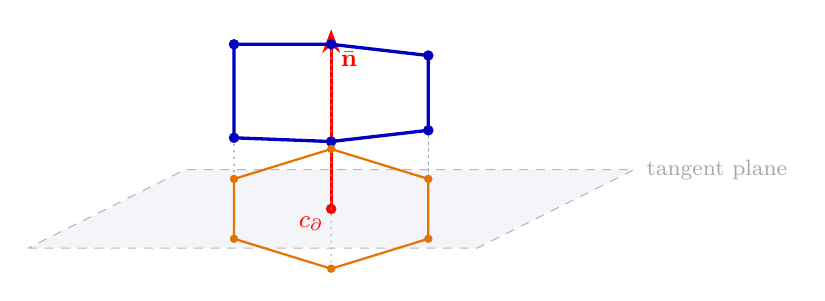
\begin{tikzpicture}[scale=0.95, line join=round, line cap=round]
        \pgfmathsetmacro{\sx}{0.7}
        \pgfmathsetmacro{\sy}{0.35}
        \coordinate (A) at (-3.0, 0);
        \coordinate (B) at ( 3.0, 0);
        \coordinate (C) at ($(B) + (\sx*3, \sy*3)$);
        \coordinate (D) at ($(A) + (\sx*3, \sy*3)$);
        \fill[ackblue!6] (A) -- (B) -- (C) -- (D) -- cycle;
        \draw[gray!55, dashed] (A) -- (B) -- (C) -- (D) -- cycle;
        \node[gray!70, font=\footnotesize, right=1pt] at (C) {tangent plane};
        \coordinate (c) at ($0.5*(A) + 0.5*(C)$);
        \fill[red] (c) circle (2pt);
        \node[red, font=\small, below left=-1pt] at (c) {$c_{\partial}$};
        \draw[-{Stealth[length=3mm]}, very thick, red] (c) -- ++(0, 2.4);
        \node[red, font=\small, right] at ($(c) + (0, 2.0)$) {$\bar{\mathbf{n}}$};
        \foreach \i/\ang/\dz in {0/30/0.55, 1/90/0.30, 2/150/0.70, 3/210/0.25, 4/270/0.60, 5/330/0.35} {
            \pgfmathsetmacro{\ang}{60*\i + 30}
            \coordinate (p\i) at ($(c) + ({1.5*cos(\ang)}, {0.8*sin(\ang)})$);
            \coordinate (v\i) at ($(p\i) + (0, {1.1 + \dz})$);
        }
        \foreach \i in {0,...,5} {
            \draw[dotted, gray!70] (v\i) -- (p\i);
        }
        \draw[very thick, blue!75!black]
            (v0) -- (v1) -- (v2) -- (v3) -- (v4) -- (v5) -- cycle;
        \foreach \i in {0,...,5} { \fill[blue!75!black] (v\i) circle (2pt); }
        \draw[thick, orange!90!black]
            (p0) -- (p1) -- (p2) -- (p3) -- (p4) -- (p5) -- cycle;
        \foreach \i in {0,...,5} { \fill[orange!90!black] (p\i) circle (1.6pt); }
    \end{tikzpicture}
    \caption{Projection of the 3D boundary (blue) onto the tangent plane defined by $\bar{\mathbf{n}}$.}
    \label{fig:2d-projection}
\end{figure}

\subsection*{Ear clipping}

The naive version of ear clipping picks the first valid ear at each step, which on a regular polygon degenerates into a fan of sliver triangles (Figure~\ref{fig:ear-clipping}, left). The implementation scans every valid ear at each step and picks the one whose minimum interior angle is largest. This produces a noticeably more even tessellation. Three fallback layers handle pathological input: if no valid ear exists, the first convex vertex is clipped; if no convex vertex exists, vertex 1 is force-clipped; if the polygon collapses below three vertices, the loop stops. A winding check against $\bar{\mathbf{n}}$ at the end flips the triangle ordering if the patch ended up facing the wrong way.

The first version of this stage used FIFO ear selection. The patch on \texttt{sphere\_small} came out as a fan of slivers concentrated at one vertex, and downstream this caused Stage~4 to produce visibly biased normals near that vertex. Switching the heuristic to max-min interior angle was a five-line change and removed the bias.

\begin{figure}[H]
    \centering
    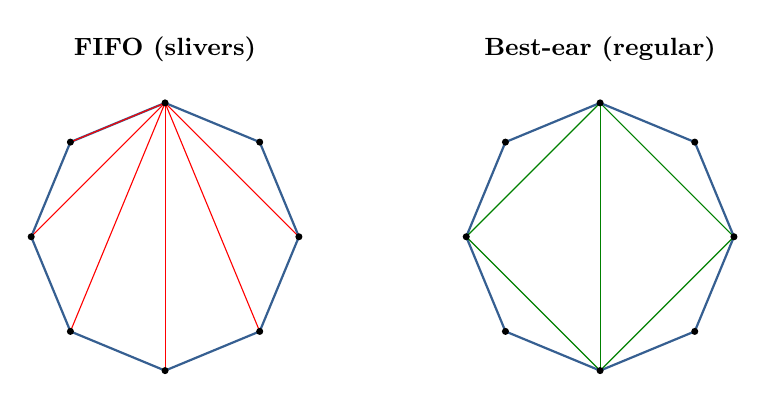
\begin{tikzpicture}[scale=0.85, line join=round]
        \begin{scope}[xshift=0cm]
            \node[font=\small\bfseries] at (0, 2.8) {FIFO (slivers)};
            \foreach \i/\lbl in {0/p_0, 1/p_1, 2/p_2, 3/p_3, 4/p_4, 5/p_5, 6/p_6, 7/p_7} {
                \coordinate (fan\i) at ({360/8 * \i + 90}:2);
            }
            \draw[thick, ackblue]
                (fan0) -- (fan1) -- (fan2) -- (fan3) -- (fan4) --
                (fan5) -- (fan6) -- (fan7) -- cycle;
            \foreach \i in {1,2,3,4,5,6} { \draw[red, thin] (fan0) -- (fan\i); }
            \foreach \i in {0,...,7} { \fill (fan\i) circle (1.5pt); }
        \end{scope}
        \begin{scope}[xshift=6.5cm]
            \node[font=\small\bfseries] at (0, 2.8) {Best-ear (regular)};
            \foreach \i in {0,...,7} { \coordinate (be\i) at ({360/8 * \i + 90}:2); }
            \draw[thick, ackblue]
                (be0) -- (be1) -- (be2) -- (be3) -- (be4) --
                (be5) -- (be6) -- (be7) -- cycle;
            \draw[green!50!black, thin] (be0) -- (be2);
            \draw[green!50!black, thin] (be2) -- (be4);
            \draw[green!50!black, thin] (be4) -- (be6);
            \draw[green!50!black, thin] (be6) -- (be0);
            \draw[green!50!black, thin] (be0) -- (be4);
            \foreach \i in {0,...,7} { \fill (be\i) circle (1.5pt); }
        \end{scope}
    \end{tikzpicture}
    \caption{FIFO ear clipping (left) versus best-ear clipping (right) on the same polygon.}
    \label{fig:ear-clipping}
\end{figure}

\subsection*{Delaunay flips and centroid refinement}

For each interior edge shared by two triangles, the alternate diagonal is considered as a flip candidate. The flip is accepted only if it strictly increases the minimum interior angle across the pair. A face that has already been flipped in the current pass is locked until the next one, which prevents conflicting flips during a single sweep. On the test meshes, three passes are enough to converge.

The flip pass was the part of Stage~3 that took longest to get right. The issue was deriving the correct winding for the new diagonal on a curved 3D patch: a global sign-check against $\bar{\mathbf{n}}$ works for nearly planar patches but breaks once the patch curves enough that the new triangle faces the opposite side of $\bar{\mathbf{n}}$ from the original. After being stuck on this for an hour or two, going back to the lecture material on mesh orientation gave the right hint --- the cyclic order of $u, v$ inside the original triangle $t_1$ already encodes the orientation locally, so no global vector is needed. The two-case split in the code (whether $t_1$ contains $u \to v$ or $v \to u$) is the consequence.

\begin{figure}[H]
    \centering
    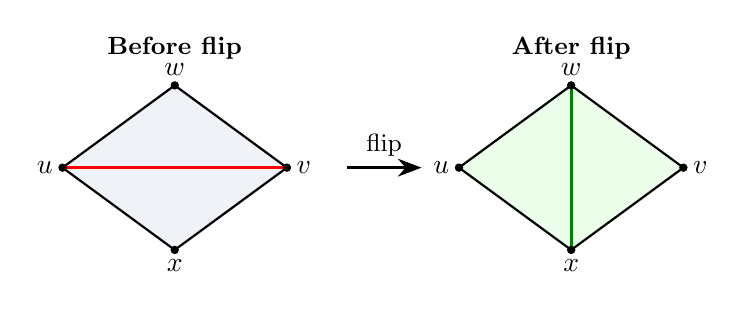
\begin{tikzpicture}[scale=0.95, line join=round]
        \begin{scope}[xshift=0cm]
            \node[font=\small\bfseries] at (1.5, 3.1) {Before flip};
            \coordinate (u) at (0, 1.5); \coordinate (v) at (3, 1.5);
            \coordinate (w) at (1.5, 2.6); \coordinate (x) at (1.5, 0.4);
            \fill[ackblue!8] (u) -- (v) -- (w) -- cycle;
            \fill[ackblue!8] (u) -- (v) -- (x) -- cycle;
            \draw[thick] (u) -- (w) -- (v) -- (x) -- cycle;
            \draw[red, very thick] (u) -- (v);
            \fill (u) circle (1.6pt); \node[left]  at (u) {$u$};
            \fill (v) circle (1.6pt); \node[right] at (v) {$v$};
            \fill (w) circle (1.6pt); \node[above] at (w) {$w$};
            \fill (x) circle (1.6pt); \node[below] at (x) {$x$};
        \end{scope}
        \draw[-{Stealth[length=3mm]}, very thick]
            (3.8, 1.5) -- (4.8, 1.5) node[midway, above, font=\small] {flip};
        \begin{scope}[xshift=5.3cm]
            \node[font=\small\bfseries] at (1.5, 3.1) {After flip};
            \coordinate (u) at (0, 1.5); \coordinate (v) at (3, 1.5);
            \coordinate (w) at (1.5, 2.6); \coordinate (x) at (1.5, 0.4);
            \fill[green!8] (u) -- (w) -- (x) -- cycle;
            \fill[green!8] (v) -- (w) -- (x) -- cycle;
            \draw[thick] (u) -- (w) -- (v) -- (x) -- cycle;
            \draw[green!50!black, very thick] (w) -- (x);
            \fill (u) circle (1.6pt); \node[left]  at (u) {$u$};
            \fill (v) circle (1.6pt); \node[right] at (v) {$v$};
            \fill (w) circle (1.6pt); \node[above] at (w) {$w$};
            \fill (x) circle (1.6pt); \node[below] at (x) {$x$};
        \end{scope}
    \end{tikzpicture}
    \caption{Edge flip replaces diagonal $(u,v)$ with $(w,x)$ when this increases the minimum angle.}
    \label{fig:delaunay-flip}
\end{figure}

The target triangle area is set to that of an equilateral triangle with side $\bar{e} \cdot \texttt{RefinementFactor}$, where $\bar{e}$ is the average boundary edge length. Faces with area above $1.5 \times$ the target are split by inserting their centroid as a new interior vertex. Up to eight refinement passes run, capped at 200\,000 faces total to prevent runaway subdivision on aggressive parameter values. A second Delaunay flip pass cleans up slivers introduced by centroid insertion.

\section{Normal field diffusion}

This is the stage that gives the patch its curvature. Each component of the vertex normal is treated as a scalar field on the patch, the boundary values are pinned to those from Stage~2, and the heat equation is used to propagate boundary information inward. The continuous problem is
\begin{equation}
\frac{\partial \mathbf{n}}{\partial t} = \lambda \, \Delta_\Omega \mathbf{n}, \qquad \mathbf{n}\big|_{\partial\Omega} = \mathbf{n}^{\text{fixed}},
\end{equation}
applied component-wise. The steady state is the harmonic extension of the boundary normals into the patch interior.

\begin{figure}[H]
    \centering
    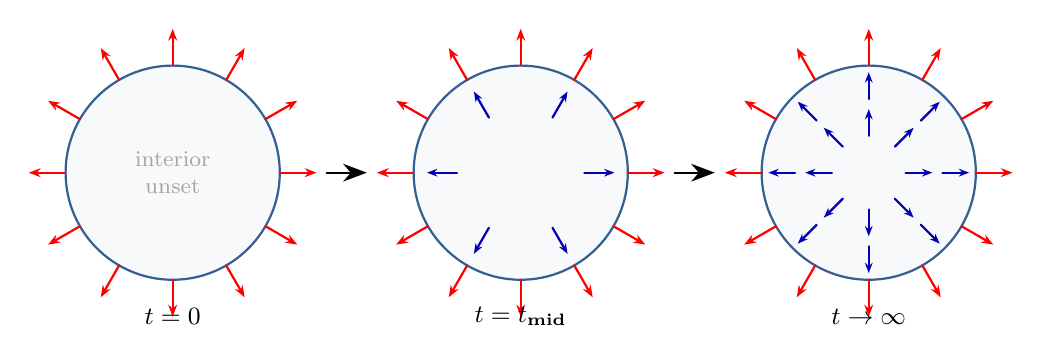
\begin{tikzpicture}[scale=0.85, line join=round, line cap=round]
        \pgfmathsetmacro{\R}{1.6}
        \tikzset{bnd/.style={-{Stealth[length=1.5mm]}, red, thick}}
        \tikzset{intarr/.style={-{Stealth[length=1.3mm]}, blue!70!black, thick}}
        \begin{scope}[xshift=0cm]
            \draw[thick, ackblue, fill=ackblue!4] (0, 0) circle (\R);
            \foreach \ang in {0, 30, 60, 90, 120, 150, 180, 210, 240, 270, 300, 330} {
                \draw[bnd] ({\R*cos(\ang)}, {\R*sin(\ang)})
                        -- ({(\R+0.55)*cos(\ang)}, {(\R+0.55)*sin(\ang)});
            }
            \node[gray!70, font=\footnotesize, align=center] at (0, 0) {interior\\unset};
            \node[font=\small\bfseries] at (0, -\R - 0.55) {$t = 0$};
        \end{scope}
        \begin{scope}[xshift=5.2cm]
            \draw[thick, ackblue, fill=ackblue!4] (0, 0) circle (\R);
            \foreach \ang in {0, 30, 60, 90, 120, 150, 180, 210, 240, 270, 300, 330} {
                \draw[bnd] ({\R*cos(\ang)}, {\R*sin(\ang)})
                        -- ({(\R+0.55)*cos(\ang)}, {(\R+0.55)*sin(\ang)});
            }
            \foreach \ang in {0, 60, 120, 180, 240, 300} {
                \draw[intarr] ({0.95*cos(\ang)}, {0.95*sin(\ang)})
                           -- ({(0.95+0.45)*cos(\ang)}, {(0.95+0.45)*sin(\ang)});
            }
            \node[font=\small\bfseries] at (0, -\R - 0.55) {$t = t_{\text{mid}}$};
        \end{scope}
        \begin{scope}[xshift=10.4cm]
            \draw[thick, ackblue, fill=ackblue!4] (0, 0) circle (\R);
            \foreach \ang in {0, 30, 60, 90, 120, 150, 180, 210, 240, 270, 300, 330} {
                \draw[bnd] ({\R*cos(\ang)}, {\R*sin(\ang)})
                        -- ({(\R+0.55)*cos(\ang)}, {(\R+0.55)*sin(\ang)});
            }
            \foreach \r in {0.55, 1.1} {
                \foreach \ang in {0, 45, 90, 135, 180, 225, 270, 315} {
                    \draw[intarr] ({\r*cos(\ang)}, {\r*sin(\ang)})
                               -- ({(\r+0.40)*cos(\ang)}, {(\r+0.40)*sin(\ang)});
                }
            }
            \node[font=\small\bfseries] at (0, -\R - 0.55) {$t \to \infty$};
        \end{scope}
        \draw[-{Stealth[length=3mm]}, thick] (2.3, 0) -- (2.9, 0);
        \draw[-{Stealth[length=3mm]}, thick] (7.5, 0) -- (8.1, 0);
    \end{tikzpicture}
    \caption{Heat-equation diffusion of the normal field, from initial state to harmonic steady state.}
    \label{fig:heat-diffusion}
\end{figure}

Discretising with implicit Euler gives, per component,
\begin{equation}
(I + \lambda L_{\text{cot}})\, \mathbf{n}^{t+1}_{\text{int}} = \mathbf{n}^{t}_{\text{int}} + \lambda\, \mathbf{b},
\end{equation}
where $\mathbf{b}_i = \sum_{j \in \partial \cap \mathcal{N}(i)} w_{ij}\, n_j^{\text{fixed}}$ collects the contributions from fixed boundary neighbours. This is the standard finite-element treatment of Dirichlet conditions: boundary values are eliminated from the unknown vector and reappear on the right-hand side. The system matrix is built from cotangent weights, computed face by face on the patch. Diagonal entries are $1 + \lambda \sum_j w_{ij}$, summing over \emph{all} neighbours (both interior and boundary). Off-diagonal entries are $-\lambda w_{ij}$, limited to interior neighbours.

The matrix is symmetric positive definite, sparse, and constant across iterations, so it is factored once with \texttt{Eigen::SimplicialLDLT} and reused:

\begin{algorithm}[H]
\caption{Iterative implicit Euler}
\begin{algorithmic}[1]
\State $A \gets I + \lambda L_{\text{cot}}$
\State $\texttt{solver}.\text{compute}(A)$ \Comment{$LDL^T$ factorisation, once}
\For{$t = 1$ to \texttt{DiffusionIterations}}
    \State $\text{rhs} \gets \mathbf{n}^{t}_{\text{int}} + \lambda\, \mathbf{b}$
    \State $\mathbf{n}^{t+1}_{\text{int}} \gets \texttt{solver}.\text{solve}(\text{rhs})$
\EndFor
\State Normalise each $\mathbf{n}_i$
\end{algorithmic}
\end{algorithm}

The default of 50 iterations is sufficient for visual convergence on the test meshes. After the loop, each diffused normal is normalised to unit length, with a guard for the rare zero-magnitude case. A separate NaN check in the caller catches any non-finite component (which can occur on extremely degenerate cotangent weights) and resets the interior normals to the boundary average.

\section{Laplacian smoothing}

Stage~5 redistributes the interior vertex \emph{positions} on the still-flat patch using uniform Laplacian smoothing,
\begin{equation}
v_i^{(k+1)} = \frac{1}{|\mathcal{N}(v_i)|} \sum_{v_j \in \mathcal{N}(v_i)} v_j^{(k)},
\end{equation}
with boundary vertices held fixed. The uniform Laplacian is appropriate here because the goal is to even out vertex spacing on a flat surface, not to approximate a continuous operator. The default is three iterations.

\section{Curvature-guided displacement}

This stage bends the flat patch into a dome. The displacement amplitude at the dome apex is estimated from the boundary geometry by fitting an imaginary spherical cap. The cap radius is
\begin{equation}
r = \tfrac{1}{|\partial|} \sum_{i \in \partial} \|v_i - c_\partial\|,
\end{equation}
the boundary's mean distance from its centroid, and the half-angle is
\begin{equation}
\theta = \arccos\Big( \tfrac{1}{|\partial|} \sum_{i} \mathbf{n}_i \cdot \bar{\mathbf{n}} \Big),
\end{equation}
the mean angle between each boundary normal and the boundary's average normal. For a hole on a sphere this is exact: a chord of length $r$ at half-angle $\theta/2$ from the cap apex gives cap height $h = r \tan(\theta/2)$. The user-facing \texttt{CurvatureStrength} parameter scales this:
\begin{equation}
h = r \, \tan(\theta/2) \cdot \texttt{CurvatureStrength}. \label{eq:cap-height}
\end{equation}

\begin{figure}[H]
    \centering
    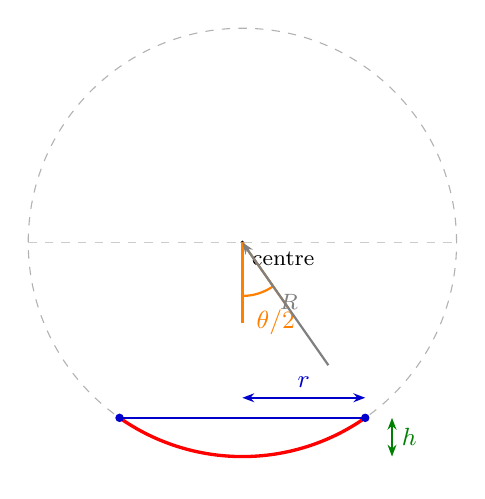
\begin{tikzpicture}[scale=1.7, line join=round]
        \pgfmathsetmacro{\Rr}{1.6}
        \pgfmathsetmacro{\halfang}{35}
        \pgfmathsetmacro{\capL}{-90 + \halfang}
        \pgfmathsetmacro{\chordY}{-\Rr * cos(\halfang)}
        \pgfmathsetmacro{\topY}{-\Rr}
        \pgfmathsetmacro{\chordX}{\Rr * sin(\halfang)}
        \draw[dashed, gray!60] (0, 0) circle (\Rr);
        \draw[dashed, gray!40] (-\Rr, 0) -- (\Rr, 0);
        \fill (0, 0) circle (0.4pt);
        \node[below right, font=\footnotesize] at (0, 0) {centre};
        \draw[very thick, red]
            (\chordX, \chordY) arc[start angle=\capL, end angle=-90-\halfang, radius=\Rr];
        \draw[thick, blue!80!black] (-\chordX, \chordY) -- (\chordX, \chordY);
        \draw[{Stealth[length=1.5mm]}-{Stealth[length=1.5mm]}, thick, green!50!black]
            (\chordX + 0.2, \chordY) -- (\chordX + 0.2, \topY);
        \node[right, green!50!black, font=\small] at (\chordX + 0.2, {(\chordY + \topY)/2}) {$h$};
        \draw[{Stealth[length=1.5mm]}-{Stealth[length=1.5mm]}, thick, blue!80!black]
            (0, \chordY + 0.15) -- (\chordX, \chordY + 0.15);
        \node[above, blue!80!black, font=\small] at ({\chordX/2}, \chordY + 0.15) {$r$};
        \draw[thick, orange] (0, 0) -- (0, -0.6);
        \draw[thick, orange] (0, 0) -- ({0.6 * sin(\halfang)}, {-0.6 * cos(\halfang)});
        \draw[thick, orange]
            ({0.4 * sin(0)}, {-0.4 * cos(0)}) arc[start angle=-90, end angle=\capL, radius=0.4];
        \node[orange, font=\small] at (0.25, -0.6) {$\theta/2$};
        \draw[{Stealth[length=1.5mm]}-, thick, gray]
            (0, 0) -- ({\Rr * sin(\halfang) * 0.7}, {-\Rr * cos(\halfang) * 0.7});
        \node[gray, font=\footnotesize] at ({\Rr * sin(\halfang) * 0.4 - 0.02}, {-\Rr * cos(\halfang) * 0.4 + 0.08}) {$R$};
        \fill[blue!80!black] (-\chordX, \chordY) circle (0.9pt);
        \fill[blue!80!black] ( \chordX, \chordY) circle (0.9pt);
    \end{tikzpicture}
    \caption{Spherical-cap geometry: chord radius $r$, half-angle $\theta/2$, cap height $h = r\tan(\theta/2)$.}
    \label{fig:spherical-cap}
\end{figure}

The mean angle is used here, not the maximum. On the Bunny and the torus, a few boundary normals point in unusual directions, and using the maximum angle in those cases pushes the dome too high. The mean turns out to be much more stable across the test set.

The first version of this stage used $\theta_{\max}$. It was correct on the spheres but on one of the Bunny's six holes, a noisy boundary normal pushed $\theta_{\max}$ to nearly $\pi/2$, and the patch in that hole came out as a tall spike rising well above the surrounding surface. Plotting the per-hole boundary-normal angle distribution made the failure mode obvious, and substituting the mean was a one-line change.

The per-vertex displacement weight depends on how far each interior vertex sits from the boundary. The distance is measured as a normalised geodesic distance via multi-source Dijkstra (Figure~\ref{fig:dijkstra-distance}): $t_i = \text{dist}_i / \max_j \text{dist}_j$, so $t = 0$ at the boundary and $t = 1$ at the geodesically farthest interior vertex.

\begin{figure}[H]
    \centering
    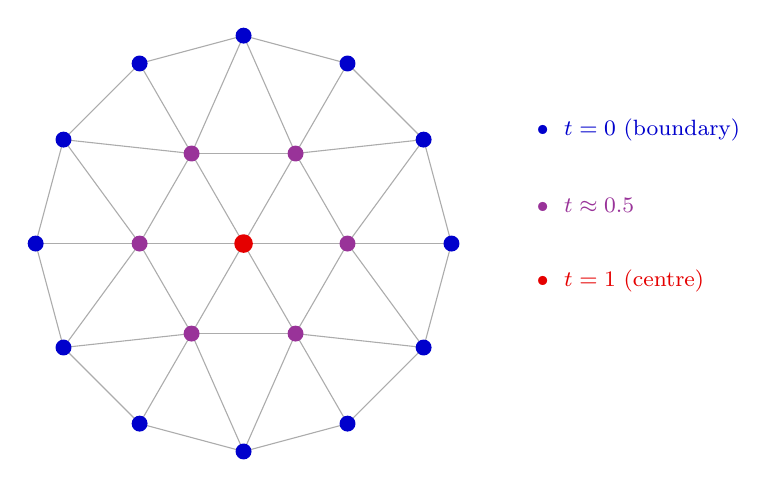
\begin{tikzpicture}[scale=1.2, line join=round]
        \pgfmathsetmacro{\Rb}{2.2}
        \pgfmathsetmacro{\Rm}{1.1}
        \foreach \i in {0,...,11} { \coordinate (b\i) at ({30*\i}:\Rb); }
        \foreach \i in {0,...,5}  { \coordinate (m\i) at ({60*\i}:\Rm); }
        \coordinate (ct) at (0, 0);
        \foreach \i in {0,...,11} {
            \pgfmathtruncatemacro{\next}{mod(\i+1, 12)}
            \draw[gray!65, thin] (b\i) -- (b\next);
        }
        \foreach \i in {0,...,5} {
            \pgfmathtruncatemacro{\next}{mod(\i+1, 6)}
            \draw[gray!65, thin] (m\i) -- (m\next);
        }
        \foreach \i in {0,...,5} { \draw[gray!65, thin] (ct) -- (m\i); }
        \foreach \i in {0,...,5} {
            \pgfmathtruncatemacro{\bal}{2*\i}
            \pgfmathtruncatemacro{\bnext}{mod(2*\i + 1, 12)}
            \pgfmathtruncatemacro{\bprev}{mod(2*\i + 11, 12)}
            \draw[gray!65, thin] (m\i) -- (b\bal);
            \draw[gray!65, thin] (m\i) -- (b\bnext);
            \draw[gray!65, thin] (m\i) -- (b\bprev);
        }
        \foreach \i in {0,...,11} { \fill[blue!80!black] (b\i) circle (2.4pt); }
        \foreach \i in {0,...,5}  { \fill[violet!80]      (m\i) circle (2.4pt); }
        \fill[red!90!black] (ct) circle (2.8pt);
        \node[blue!80!black, font=\footnotesize, right] at (3.0,  1.2) {$\bullet \ \ t = 0$ (boundary)};
        \node[violet!80,    font=\footnotesize, right] at (3.0,  0.4) {$\bullet \ \ t \approx 0.5$};
        \node[red!90!black, font=\footnotesize, right] at (3.0, -0.4) {$\bullet \ \ t = 1$ (centre)};
    \end{tikzpicture}
    \caption{Normalised geodesic distance $t$ on a triangulated patch.}
    \label{fig:dijkstra-distance}
\end{figure}

The weighting profile is
\begin{equation}
w(t) = \sqrt{2t - t^2}, \qquad t \in [0, 1]. \label{eq:profile}
\end{equation}
Geometrically, this is the height of the unit hemisphere as a function of horizontal offset, which is consistent with the spherical-cap assumption. The more important property is $w'(0) = +\infty$: the tangent is vertical at $t = 0$, so the patch tangent at the boundary is parallel to the tangent plane of the surrounding mesh, giving approximate $C^1$ continuity. A parabolic profile $4t(1-t)$ has $w'(0) = 4$ and produces a visible crease where the patch meets the surface. Figure~\ref{fig:profile-comparison} compares both.

\begin{figure}[H]
    \centering
    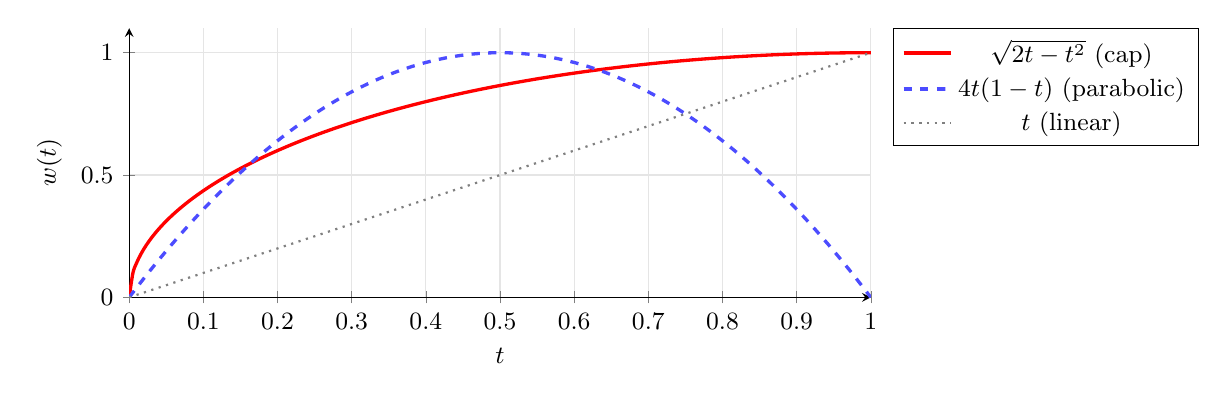
\begin{tikzpicture}
        \begin{axis}[
            width=11cm, height=5cm,
            xlabel={$t$}, ylabel={$w(t)$},
            domain=0:1, samples=200,
            xmin=0, xmax=1, ymin=0, ymax=1.1,
            axis lines=left, grid=both,
            grid style={gray!20, thin},
            legend pos=outer north east,
            legend style={font=\small},
            font=\small, no markers, smooth,
        ]
            \addplot[red, very thick] {sqrt(2*x - x*x)};
            \addlegendentry{$\sqrt{2t - t^2}$ (cap)}
            \addplot[blue!70, very thick, dashed] {4*x*(1 - x)};
            \addlegendentry{$4t(1-t)$ (parabolic)}
            \addplot[gray, thick, dotted] {x};
            \addlegendentry{$t$ (linear)}
        \end{axis}
    \end{tikzpicture}
    \caption{Displacement weighting profiles.}
    \label{fig:profile-comparison}
\end{figure}

The actual displacement is
\begin{equation}
v_i' = v_i + h \cdot w(t_i) \cdot \mathbf{n}_i^{\text{diff}},
\end{equation}
where the direction is the diffused normal from Stage~4, not the constant $\bar{\mathbf{n}}$. Using the spatially varying field allows the patch to bend differently on different sides, which matters on saddle-shaped boundaries.

After displacement, a few interior vertices may carry spike-like noise from irregular triangulation. Three pairs of Taubin smoothing ($\lambda = 0.40, \mu = -0.44$) clean this up: each pair is a positive (shrink) Laplacian step followed by a stronger negative (inflate) step. The combined filter attenuates high frequencies while preserving the dome.

\begin{figure}[H]
    \centering
    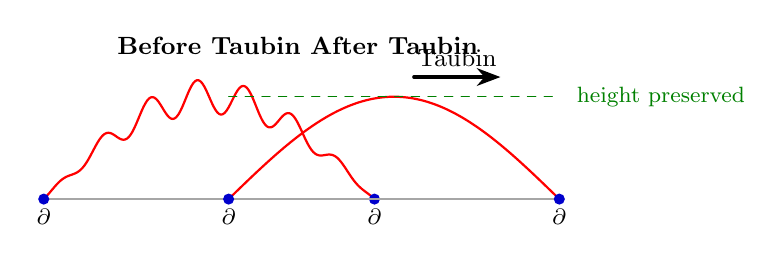
\begin{tikzpicture}[scale=1.0, line join=round, line cap=round]
        \pgfmathsetmacro{\L}{4.2}
        \pgfmathsetmacro{\H}{1.3}
        \begin{scope}[xshift=0cm]
            \draw[gray!70, thick] (0, 0) -- (\L, 0);
            \draw[red, thick, smooth, samples=180, domain=0:\L]
                plot (\x, {\H * sin(180*\x/\L)
                           + 0.22 * sin(180*14*\x/\L) * sin(180*\x/\L)});
            \fill[blue!80!black] (0, 0)  circle (2pt); \node[font=\footnotesize, below] at (0, 0)  {$\partial$};
            \fill[blue!80!black] (\L, 0) circle (2pt); \node[font=\footnotesize, below] at (\L, 0) {$\partial$};
            \node[font=\small\bfseries] at (\L/2, \H + 0.65) {Before Taubin};
        \end{scope}
        \draw[-{Stealth[length=3mm]}, very thick]
            (\L + 0.5, \H + 0.25) -- (\L + 1.6, \H + 0.25)
            node[midway, above, font=\small] {Taubin};
        \begin{scope}[xshift={\L + 2.2cm}]
            \draw[gray!70, thick] (0, 0) -- (\L, 0);
            \draw[red, thick, smooth, samples=120, domain=0:\L]
                plot (\x, {\H * sin(180*\x/\L)});
            \draw[green!50!black, dashed, thin]
                (0, \H) -- (\L, \H);
            \node[green!50!black, font=\footnotesize, right]
                at (\L, \H) {\ height preserved};
            \fill[blue!80!black] (0, 0)  circle (2pt); \node[font=\footnotesize, below] at (0, 0)  {$\partial$};
            \fill[blue!80!black] (\L, 0) circle (2pt); \node[font=\footnotesize, below] at (\L, 0) {$\partial$};
            \node[font=\small\bfseries] at (\L/2, \H + 0.65) {After Taubin};
        \end{scope}
    \end{tikzpicture}
    \caption{Taubin smoothing removes high-frequency spikes (left) without flattening the dome (right).}
    \label{fig:taubin-effect}
\end{figure}

\section{Patch merge}

The final stage stitches the patch into the host mesh. Boundary patch vertices are remapped to their original indices in $\mathcal{M}$ to avoid duplication. Interior patch vertices are appended with \texttt{AddVertices}, and faces are added with \texttt{AddFaces} after index translation. Vertex and face colours are averaged from boundary neighbours, so the patch does not appear as a white stripe on a coloured mesh. A final round of \texttt{UpdateTopology}, \texttt{UpdateNormal}, and \texttt{UpdateBounding} restores cached adjacency and attributes.

\chapter{IMPLEMENTATION}

\section{Plugin architecture}

MeshLab loads filters as dynamic libraries discovered at startup via Qt's \texttt{QPluginLoader}. A filter plugin inherits from \texttt{FilterPlugin}, is annotated with \texttt{Q\_OBJECT} and \texttt{Q\_PLUGIN\_METADATA} so the Qt MOC can wire it up, and overrides a handful of virtual methods that report metadata, declare parameters, and execute the filter. The MeshLab UI is generated automatically from the parameter list, so the only UI code needed in the plugin is the \texttt{initParameterList} call that registers the seven user parameters with their types, defaults, and tooltips.

\begin{figure}[H]
    \centering
    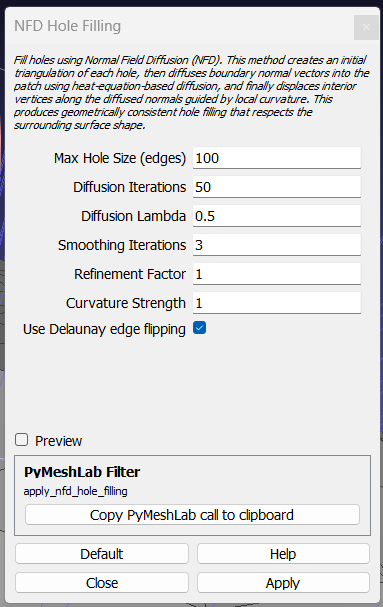
\includegraphics[width=0.5\textwidth]{figures/fig_meshlab_dialog.png}
    \caption{Filter parameter dialog generated from plugin metadata.}
    \label{fig:meshlab-dialog}
\end{figure}

The plugin is built as a CMake \texttt{MODULE} target that links against \texttt{meshlab-common}, \texttt{vcg}, and \texttt{Qt5::Core}. The output DLL goes to MeshLab's \texttt{plugins/} directory under the build tree.

\section{VCGlib usage}

VCGlib provides the mesh data structures, topology helpers, and adjacency iterators. The plugin uses:

\begin{itemize}[noitemsep]
    \item \texttt{EnableFFAdjacency} / \texttt{EnableVFAdjacency} to allocate adjacency storage on demand.
    \item \texttt{UpdateTopology::FaceFace} / \texttt{VertexFace} to populate adjacency pointers.
    \item \texttt{UpdateFlags::FaceBorderFromFF} to mark border edges, after which border tests reduce to an $O(1)$ flag query.
    \item \texttt{UpdateNormal::PerVertexNormalizedPerFace} to compute area-weighted vertex normals.
    \item \texttt{vcg::face::VFIterator} to walk the faces incident to a vertex.
    \item \texttt{vcg::tri::Allocator::AddVertices} / \texttt{AddFaces} to grow the mesh in Stage~7.
\end{itemize}

The mesh type \texttt{CMeshO} uses VCGlib's Optional Components Framework: components such as normal, colour, and adjacency are enabled per-vertex or per-face only when needed, so the storage cost matches actual usage.

\section{Eigen for the diffusion solver}

The diffusion step lives entirely in Eigen. The system matrix is built by accumulating cotangent contributions into an \texttt{Eigen::Triplet} list and committing them with \texttt{setFromTriplets}. The factorisation is one line:

\begin{lstlisting}
Eigen::SimplicialLDLT<Eigen::SparseMatrix<double>> solver;
solver.compute(A);                  // factorisation, once
for (int it = 0; it < iterations; ++it) {
    Eigen::MatrixXd rhs = ...;      // current state + boundary contribution
    normals = solver.solve(rhs);    // triangular solves, fast
}
\end{lstlisting}

\texttt{SimplicialLDLT} suits this problem: the matrix is SPD, sparse, and constant across iterations, which is exactly the factor-once / solve-many pattern the solver is built for. The boundary normals are eliminated from the unknown vector at assembly time and reappear on the right-hand side, which is the standard finite-element treatment of Dirichlet conditions.

\section{Parameters and code layout}

The seven parameters exposed to the user are summarised below. In practice, the two parameters that most often need adjustment are \texttt{CurvatureStrength} and \texttt{RefinementFactor}.

\begin{table}[H]
\centering
\caption{Plugin parameters.}
\label{tab:params}
\begin{tabularx}{\textwidth}{l l r X}
\toprule
\textbf{Parameter} & \textbf{Type} & \textbf{Default} & \textbf{Effect} \\
\midrule
\texttt{MaxHoleSize}         & int   & 100  & Skip holes longer than this. \\
\texttt{DiffusionIterations} & int   & 50   & Stage~4 iterations. \\
\texttt{DiffusionLambda}     & float & 0.5  & Stage~4 time step. \\
\texttt{SmoothingIterations} & int   & 3    & Stage~5 iterations. \\
\texttt{RefinementFactor}    & float & 1.0  & Triangle size relative to boundary edge. \\
\texttt{CurvatureStrength}   & float & 1.0  & Multiplier on cap height. \\
\texttt{UseDelaunayFlipping} & bool  & on   & Toggle Delaunay flips (off for demos). \\
\bottomrule
\end{tabularx}
\end{table}

The plugin source consists of two files: \texttt{filter\_nfd\_holefill.h} (about 70 lines, class declaration and structs) and \texttt{filter\_nfd\_holefill.cpp} (about 1\,250 lines, the full pipeline). Functions in the cpp file are laid out in pipeline order, so reading top-to-bottom follows Chapter~4. The plugin maintains no global state.

\section{Build}

The host build is MeshLab itself; the plugin is a sub-target of MeshLab's CMake project. The full build requires a one-time \texttt{cmake -G Ninja} configuration followed by \texttt{cmake --build .}\ from the MeshLab root. Incremental rebuilds of just the plugin are driven by a small batch script that calls \texttt{vcvarsall.bat x64} and rebuilds the \texttt{filter\_nfd\_holefill} target. Running MeshLab from the build tree picks up the plugin automatically.

\begin{figure}[H]
    \centering
    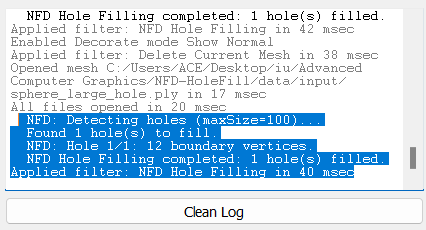
\includegraphics[width=0.85\textwidth]{figures/fig_meshlab_log.png}
    \caption{MeshLab log output after a successful filter invocation.}
    \label{fig:meshlab-log}
\end{figure}

\chapter{EXPERIMENTAL RESULTS}

\section{Test set and metric}

Evaluation is on five ground-truth meshes: two icospheres (small and large hole), a torus, the Stanford Bunny (six holes), and a watertight cow. For each model, the ground truth is paired with a holed version produced by deleting a contiguous block of faces. The test set is generated by a Python script using \texttt{trimesh} and \texttt{numpy}, with fixed random seeds for reproducibility.

\begin{table}[H]
\centering
\caption{Test models.}
\label{tab:dataset}
\begin{tabularx}{\textwidth}{l r r r X}
\toprule
\textbf{Model} & \textbf{BBox diag} & \textbf{Samples} & \textbf{Holes} & \textbf{Note} \\
\midrule
\texttt{sphere\_small} & 3.464  & 644    & 1 & Icosphere, small hole \\
\texttt{sphere\_large} & 3.464  & 652    & 1 & Icosphere, larger hole \\
\texttt{torus}         & 7.141  & 1\,920 & 1 & Hole on a curved torus section \\
\texttt{cow}           & 12.713 & 2\,911 & 1 & Large hole relative to mesh \\
\texttt{bunny}         & 0.251  & 35\,370 & 6 & Stanford Bunny, multiple holes \\
\bottomrule
\end{tabularx}
\end{table}

The metric is the symmetric Hausdorff distance computed by MeshLab's \texttt{Filters > Sampling > Hausdorff Distance}. The forward direction (filled $\to$ GT) measures how far the patch deviates from the true surface; the reverse direction (GT $\to$ filled) measures whether the patch covers the hole region. The two values capture different failure modes, so both are reported, alongside the symmetric maximum, the forward RMS, and percentages relative to the bounding-box diagonal.

\section{Hausdorff measurements}

\begin{table}[H]
\centering
\caption{Hausdorff results at default parameters. RMS is forward direction; percentages are relative to the BBox diagonal.}
\label{tab:main-results}
\begin{tabularx}{\textwidth}{l r r r r X}
\toprule
\textbf{Model} & \textbf{Sym.\ Hausd.} & \textbf{\% BBox} & \textbf{RMS (fwd)} & \textbf{RMS \%} & \textbf{Note} \\
\midrule
\texttt{sphere\_small} & $4.26 \times 10^{-3}$ & 0.123\% & $2.37 \times 10^{-4}$ & 0.007\% & --- \\
\texttt{sphere\_large} & $2.06 \times 10^{-2}$ & 0.592\% & $2.10 \times 10^{-3}$ & 0.060\% & --- \\
\texttt{torus}         & $2.45 \times 10^{-2}$ & 0.343\% & $5.60 \times 10^{-5}$ & 0.001\% & reverse-dominated \\
\texttt{cow}           & $3.32 \times 10^{-1}$ & 2.609\% & $1.44 \times 10^{-3}$ & 0.011\% & under-coverage \\
\texttt{bunny}         & $8.78 \times 10^{-3}$ & 3.498\% & $4.55 \times 10^{-4}$ & 0.181\% & one sharp hole \\
\bottomrule
\end{tabularx}
\end{table}

Spheres give the lowest error because the spherical-cap model in Stage~6 is exact for them. The factor-of-five increase from \texttt{sphere\_small} to \texttt{sphere\_large} tracks the larger hole; the relative error stays below 0.6\% in both cases.

The torus shows a different pattern. The forward RMS is very small ($5.6 \times 10^{-5}$), so the patch surface lies on the true torus, but the symmetric distance is dominated by the reverse direction. The hole crosses a strongly curved section, and a few ground-truth points near the far side of the hole have no patch vertex above them. Increasing \texttt{RefinementFactor} so the patch carries more interior vertices brings the reverse error down.

The cow shows the same reverse-direction pattern at a larger scale: $0.51\%$ forward versus $2.6\%$ reverse. The patch sits on the true surface but does not fully span the removed region along the long axis. With \texttt{RefinementFactor = 0.6} and \texttt{DiffusionIterations = 100}, the symmetric distance drops by roughly $4\times$ at about $3\times$ the runtime.

The Bunny entry shows a $3.5\%$ BBox value, but this comes from a small bounding box ($0.251$) combined with a single overshoot vertex on one of the six holes. The mean and RMS forward error are $0.02\%$ and $0.18\%$ respectively, so the rest of the patch matches the ground truth closely. Lowering \texttt{CurvatureStrength} to $0.7$ removes the spike, with the side effect of slightly flatter domes on the other five holes.

\section{Per-model figures}

\begin{figure}[H]
    \centering
    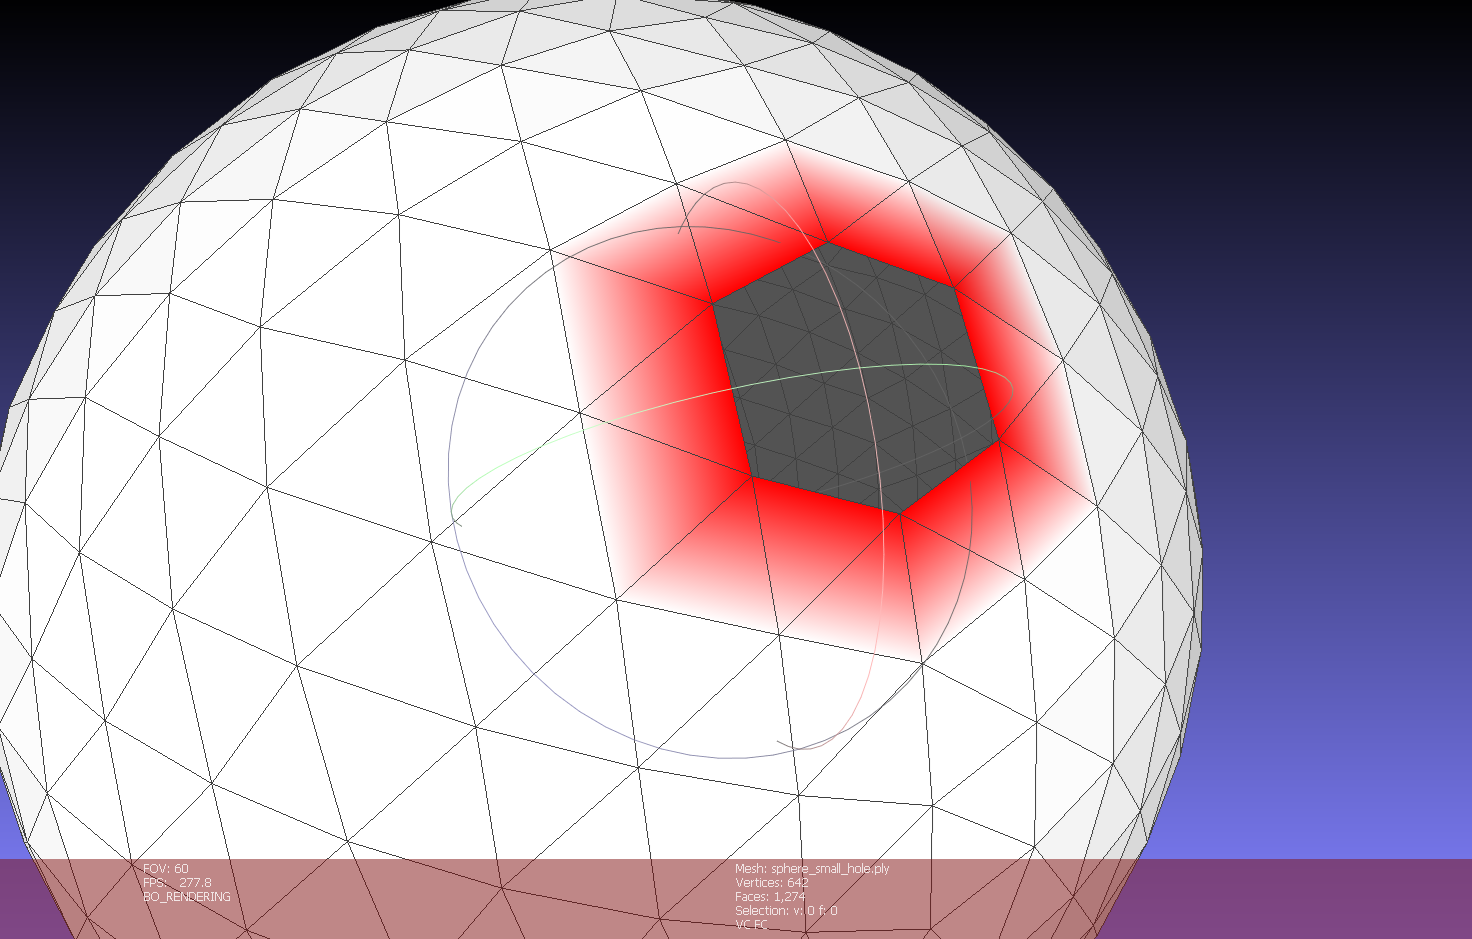
\includegraphics[width=0.45\textwidth]{figures/fig_dataset_sphere_small1.png}
    \hfill
    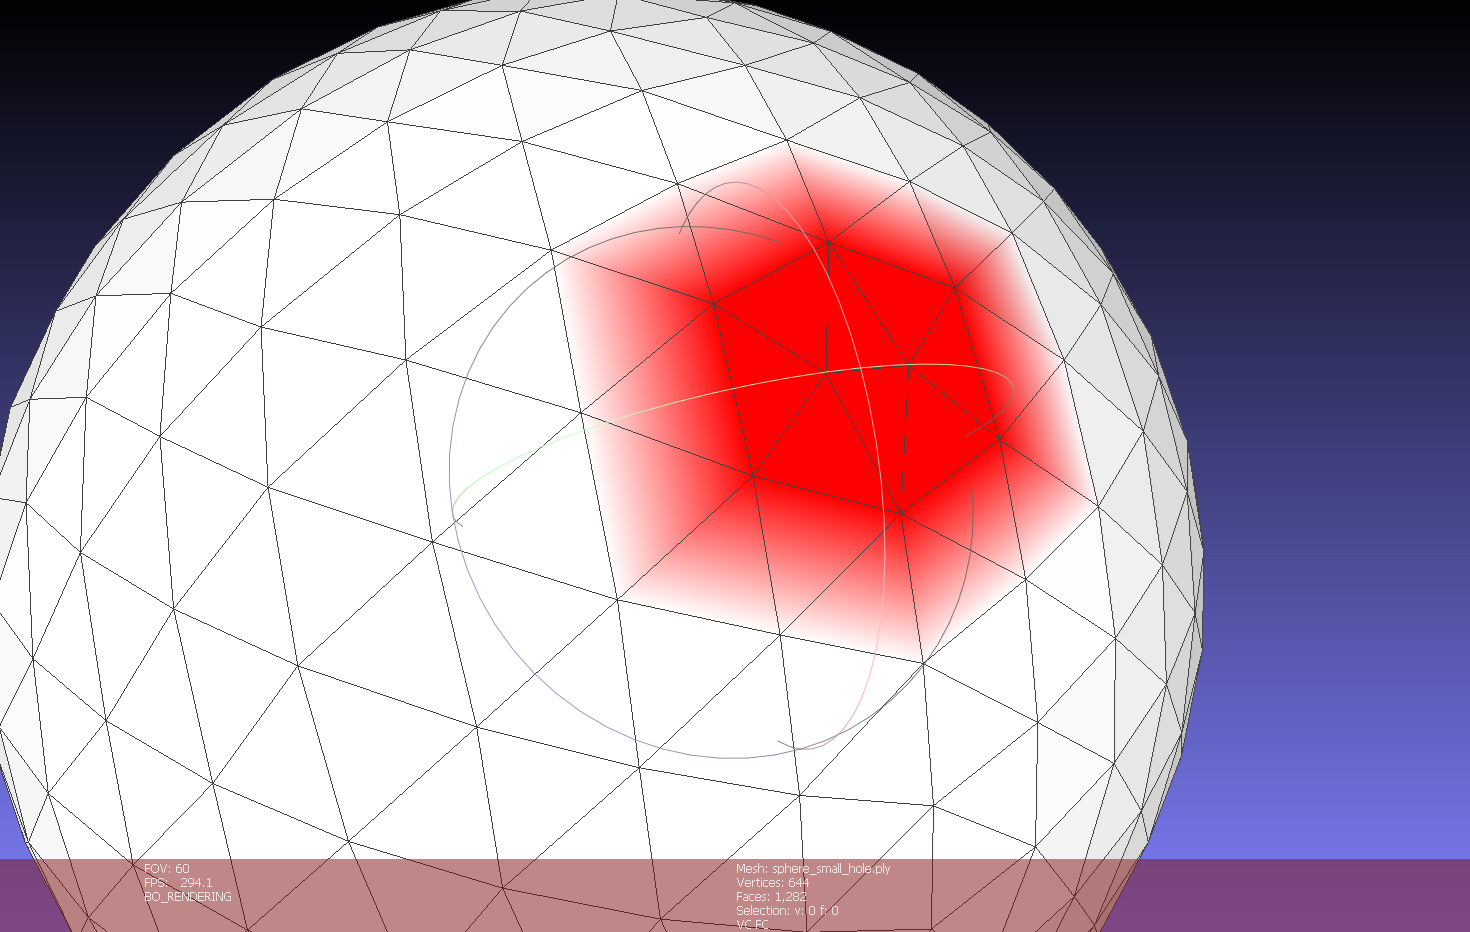
\includegraphics[width=0.45\textwidth]{figures/fig_dataset_sphere_small2.png}
    \caption{\texttt{sphere\_small}: input (left) and NFD result (right).}
    \label{fig:dataset-sphere-small}
\end{figure}

\begin{figure}[H]
    \centering
    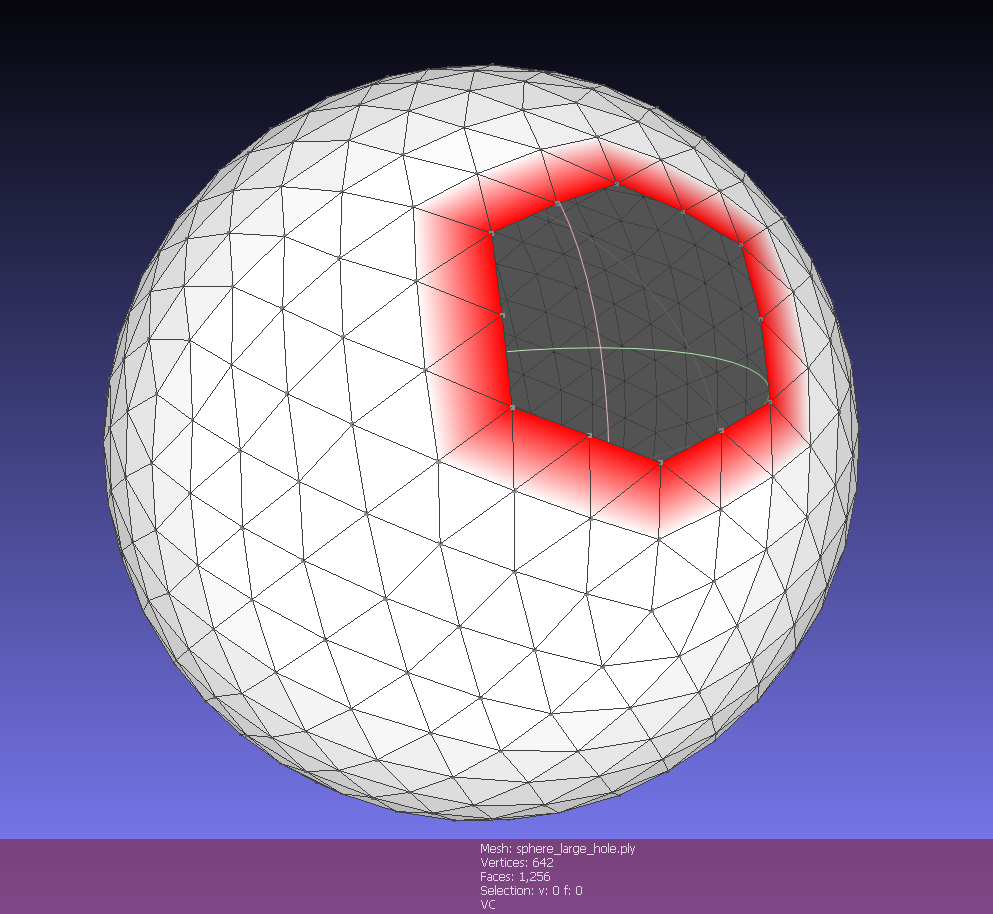
\includegraphics[width=0.45\textwidth]{figures/fig_dataset_sphere_large1.png}
    \hfill
    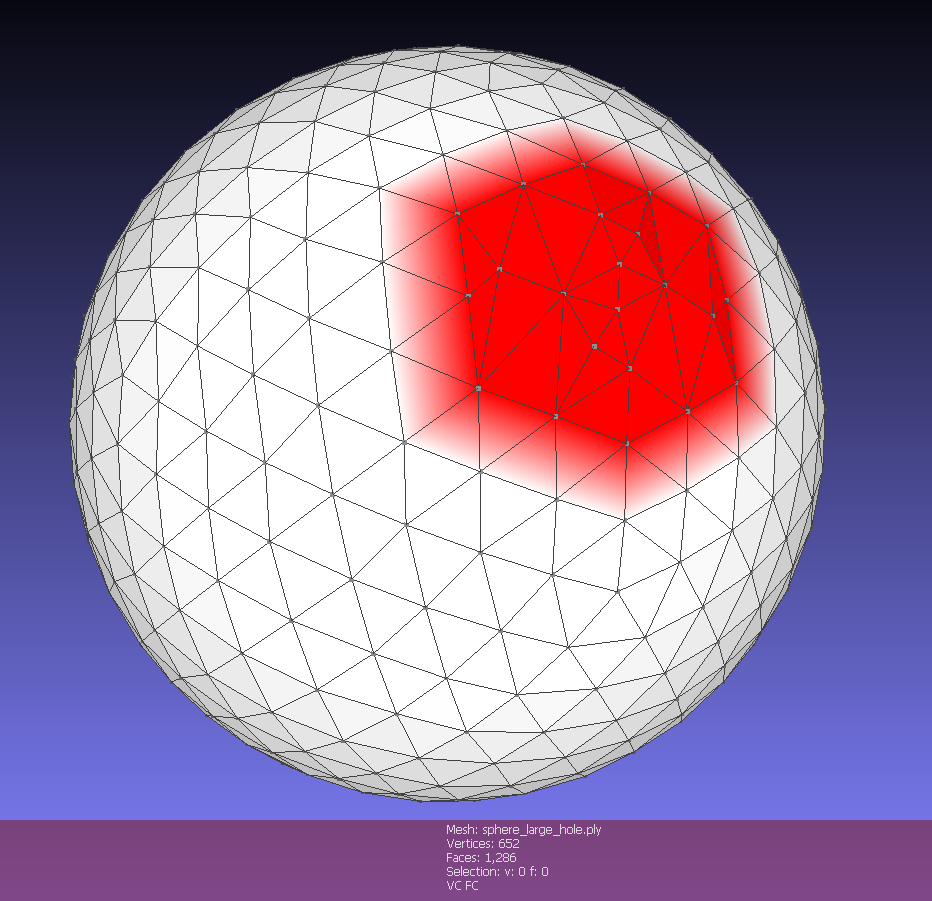
\includegraphics[width=0.45\textwidth]{figures/fig_dataset_sphere_large2.png}
    \caption{\texttt{sphere\_large}: input (left) and NFD result (right).}
    \label{fig:dataset-sphere-large}
\end{figure}

\begin{figure}[H]
    \centering
    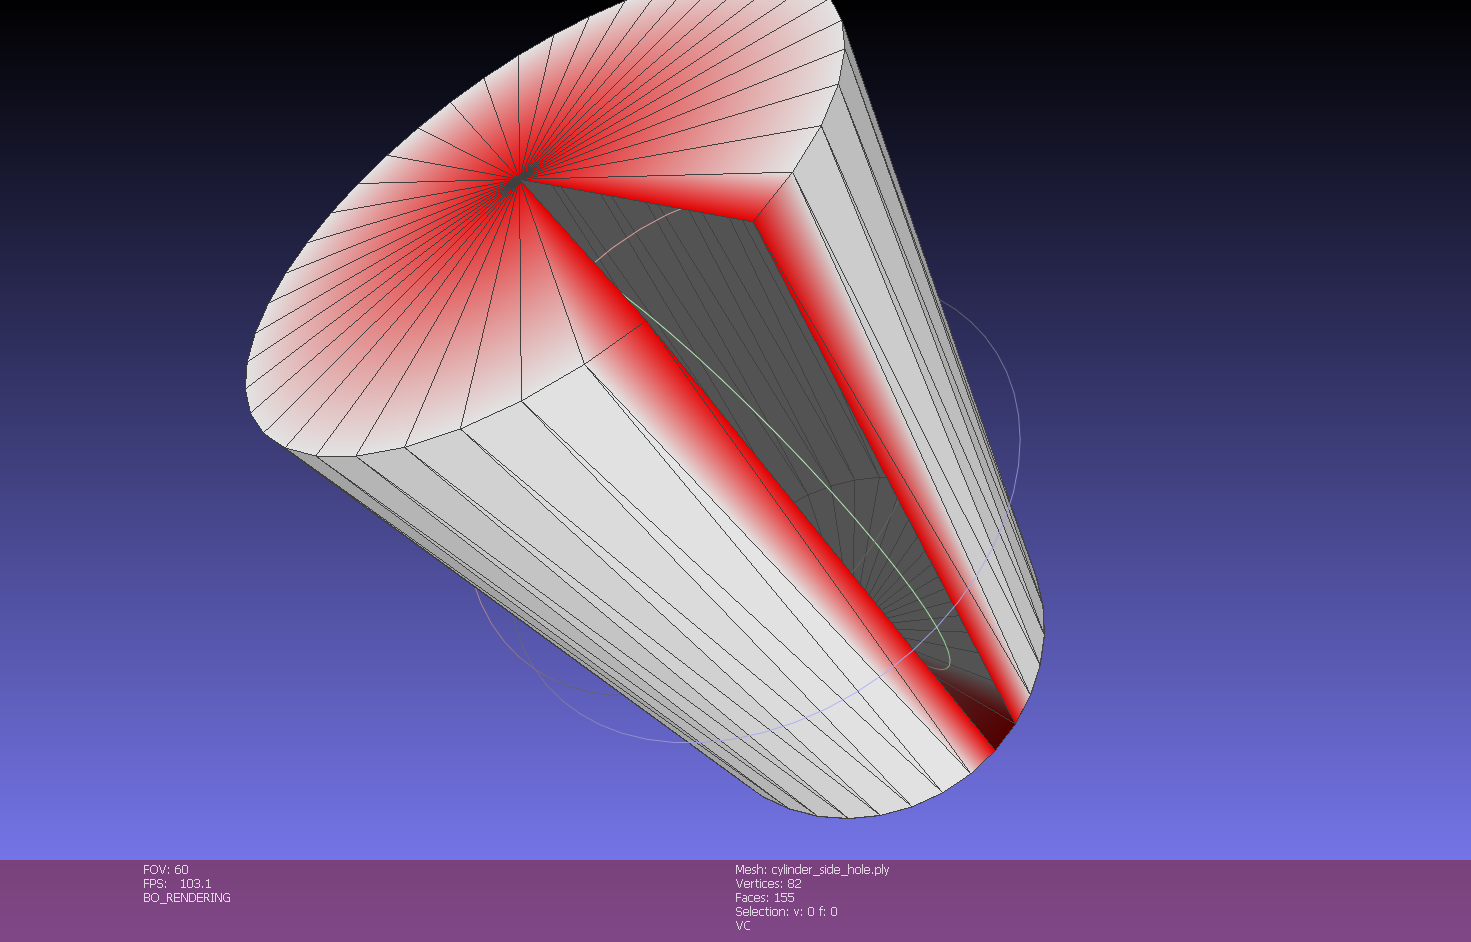
\includegraphics[width=0.45\textwidth]{figures/fig_dataset_cylinder1.png}
    \hfill
    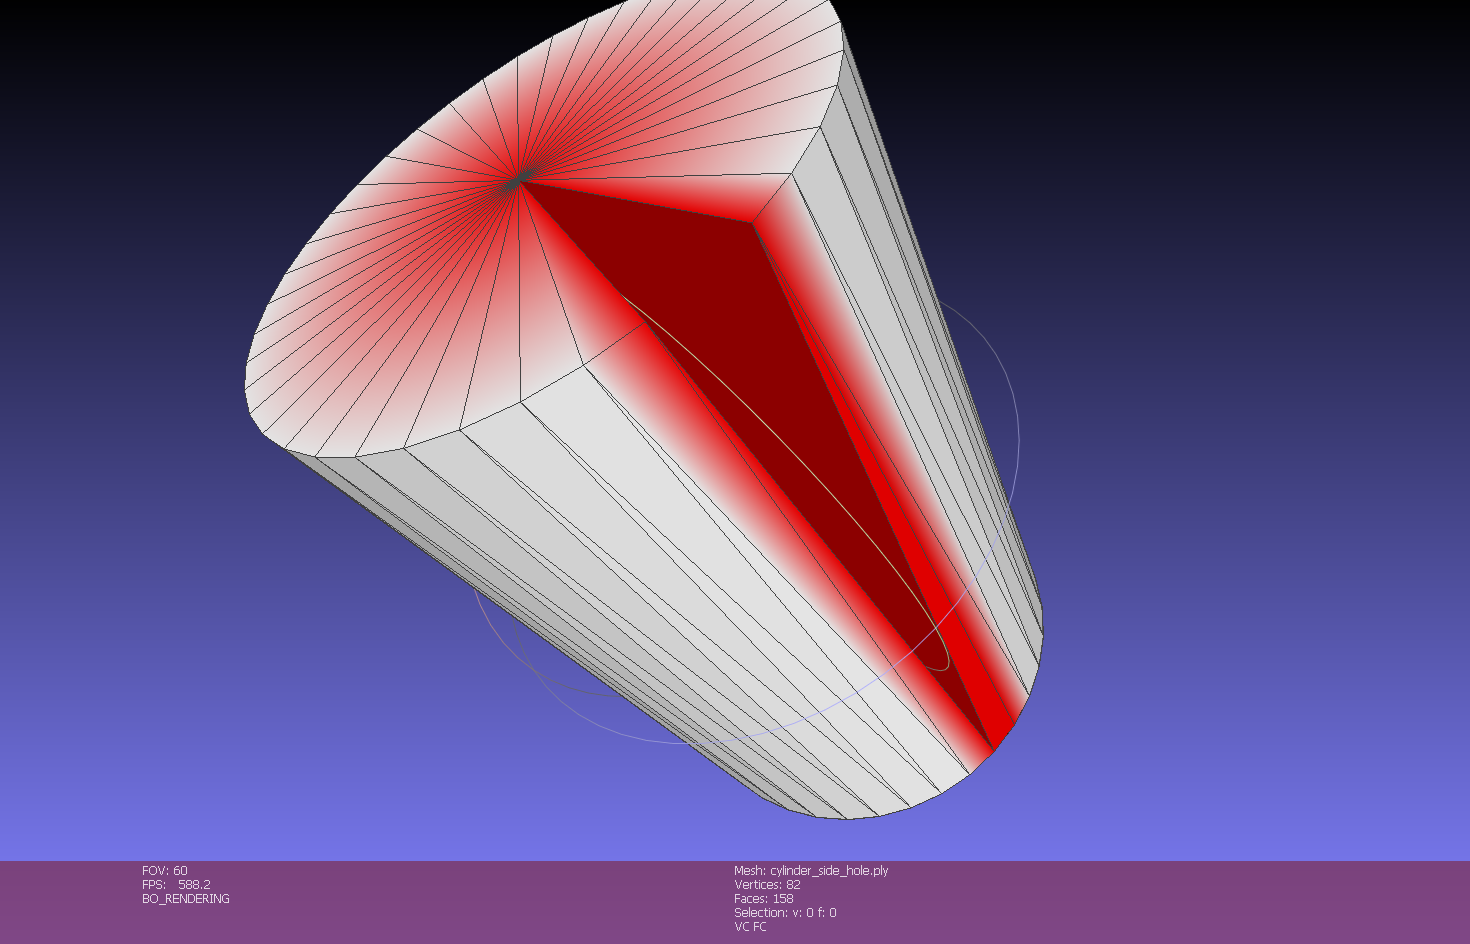
\includegraphics[width=0.45\textwidth]{figures/fig_dataset_cylinder2.png}
    \caption{\texttt{cylinder\_side}: input (left) and NFD result (right).}
    \label{fig:dataset-cylinder}
\end{figure}

\begin{figure}[H]
    \centering
    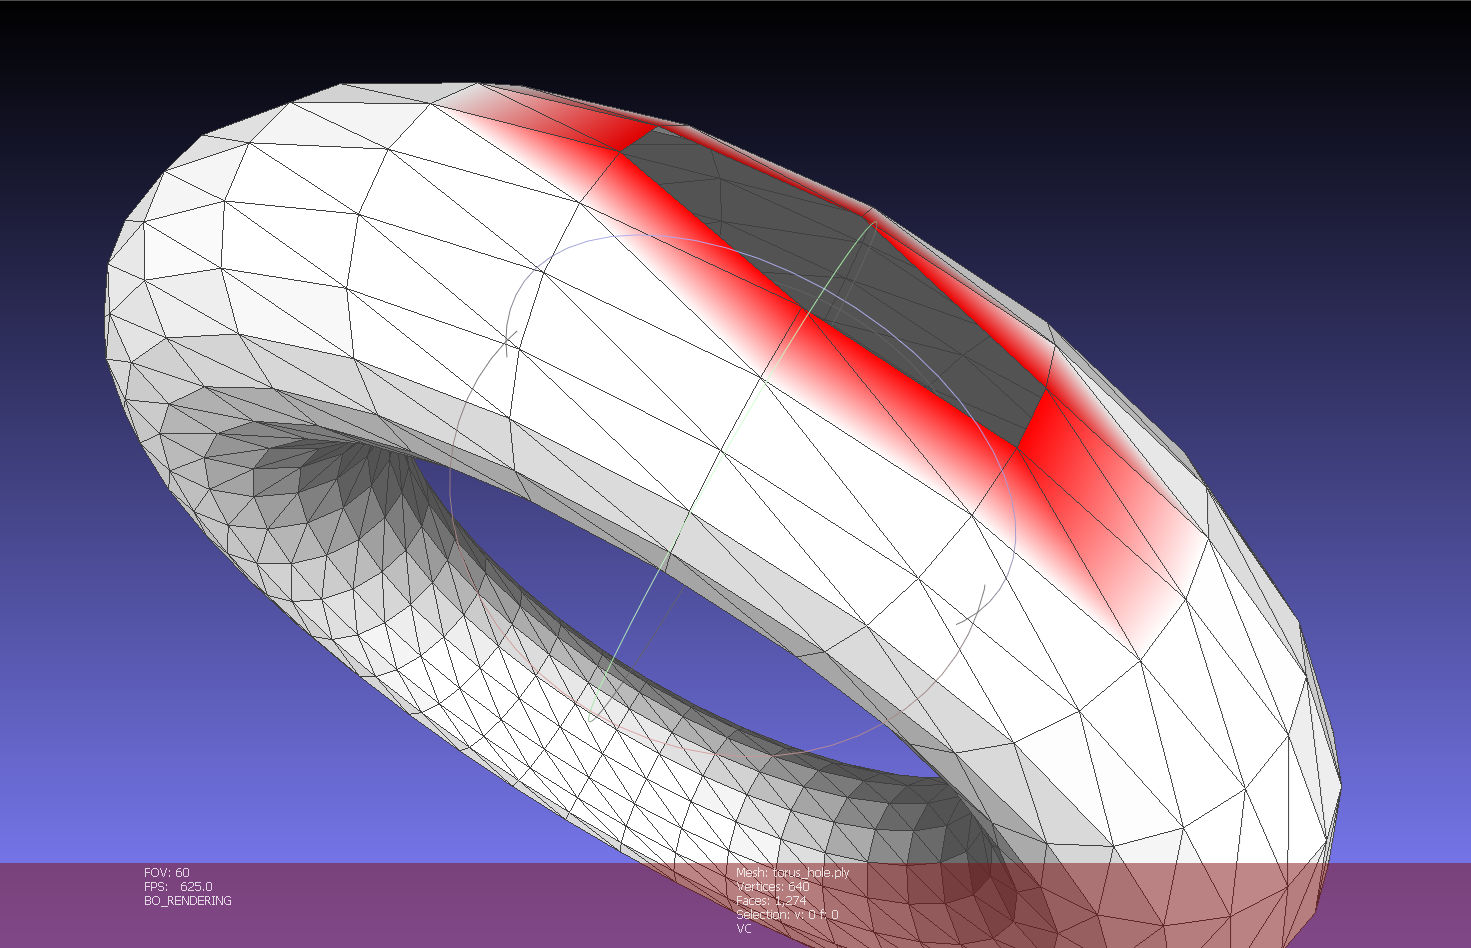
\includegraphics[width=0.45\textwidth]{figures/fig_dataset_torus1.png}
    \hfill
    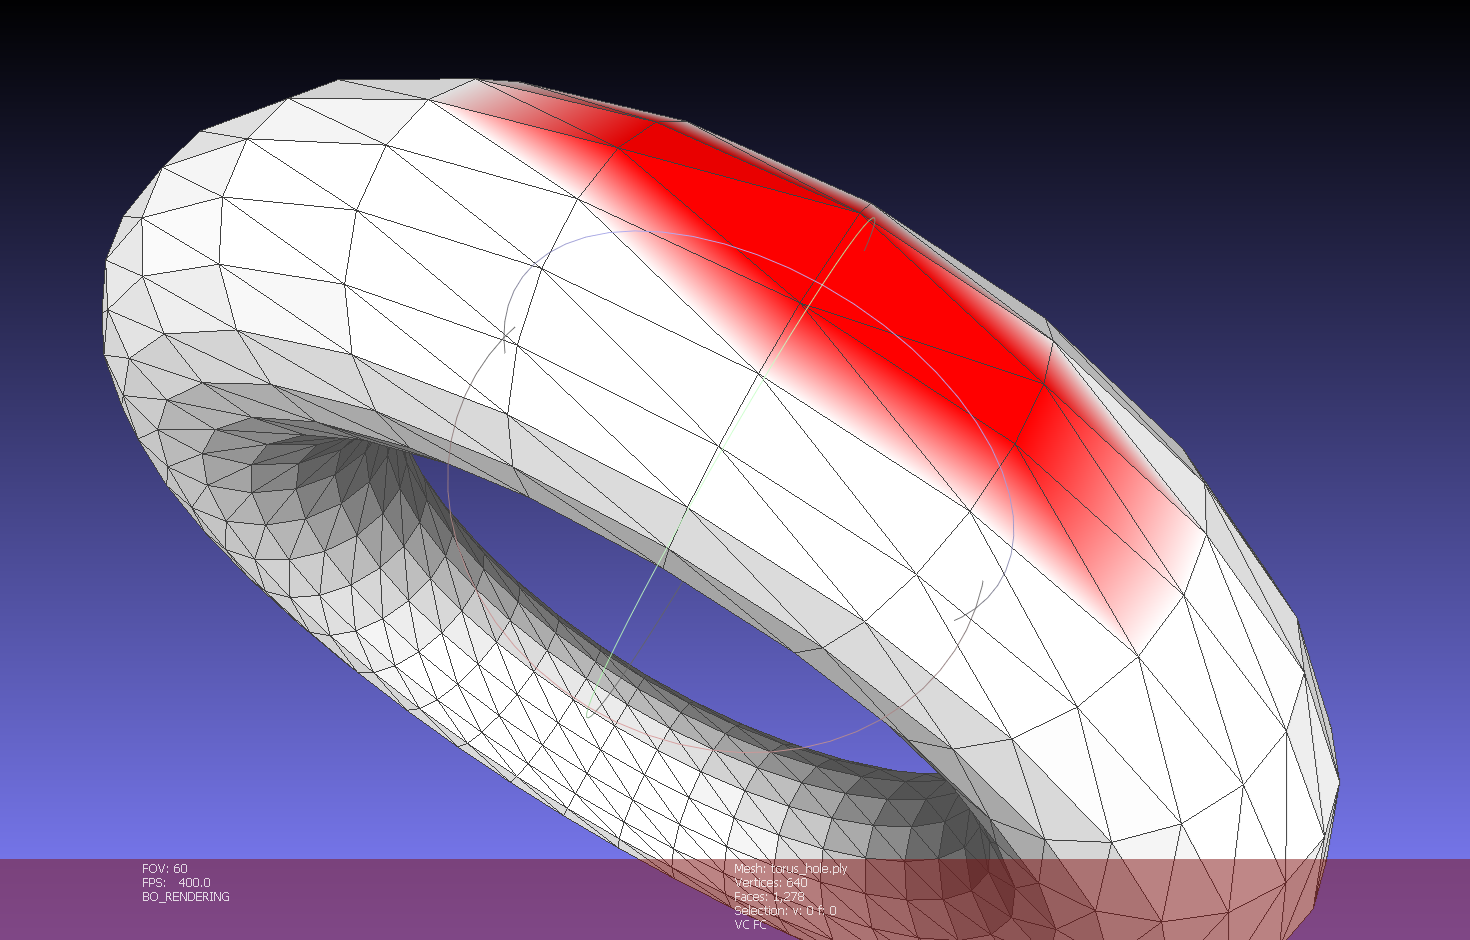
\includegraphics[width=0.45\textwidth]{figures/fig_dataset_torus2.png}
    \caption{\texttt{torus}: input (left) and NFD result (right).}
    \label{fig:dataset-torus}
\end{figure}

\begin{figure}[H]
    \centering
    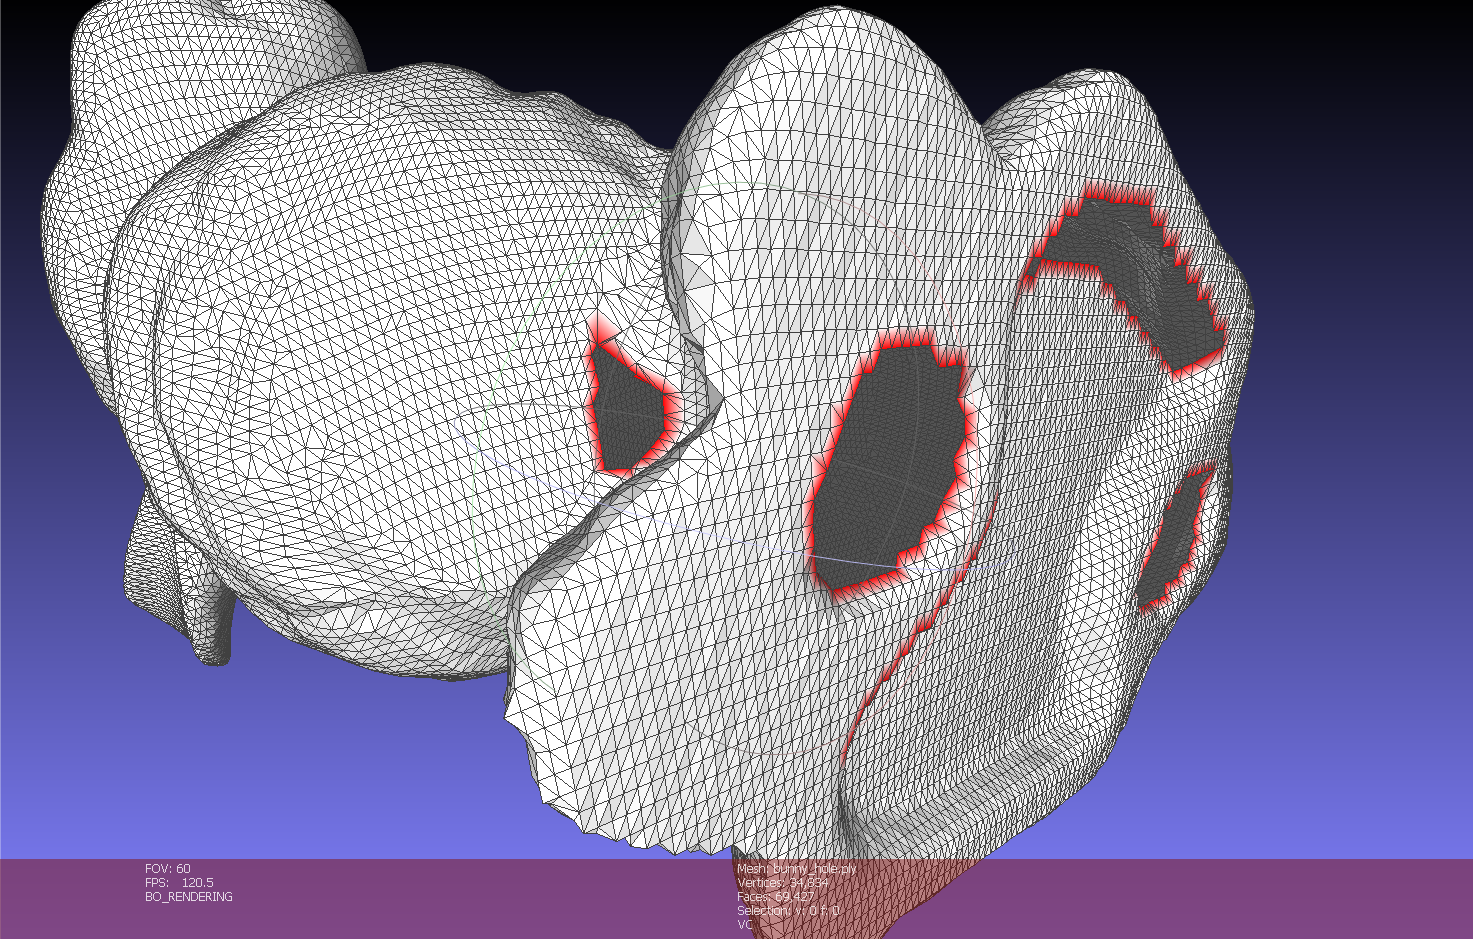
\includegraphics[width=0.45\textwidth]{figures/fig_dataset_bunny1.png}
    \hfill
    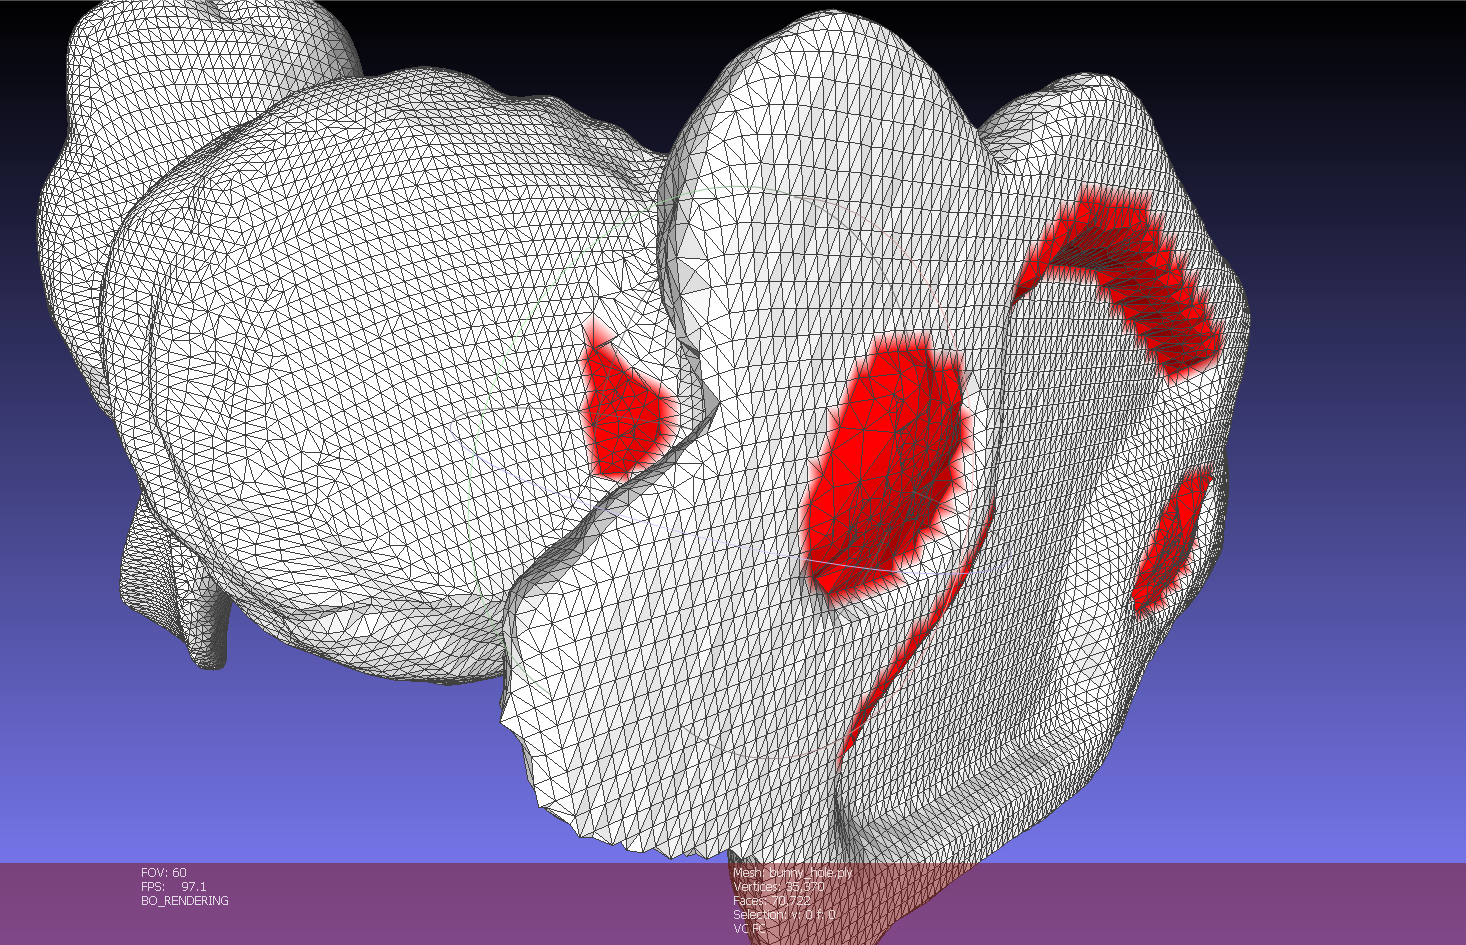
\includegraphics[width=0.45\textwidth]{figures/fig_dataset_bunny2.png}
    \caption{Stanford \texttt{bunny}: six holes (left) all filled (right).}
    \label{fig:dataset-bunny}
\end{figure}

\begin{figure}[H]
    \centering
    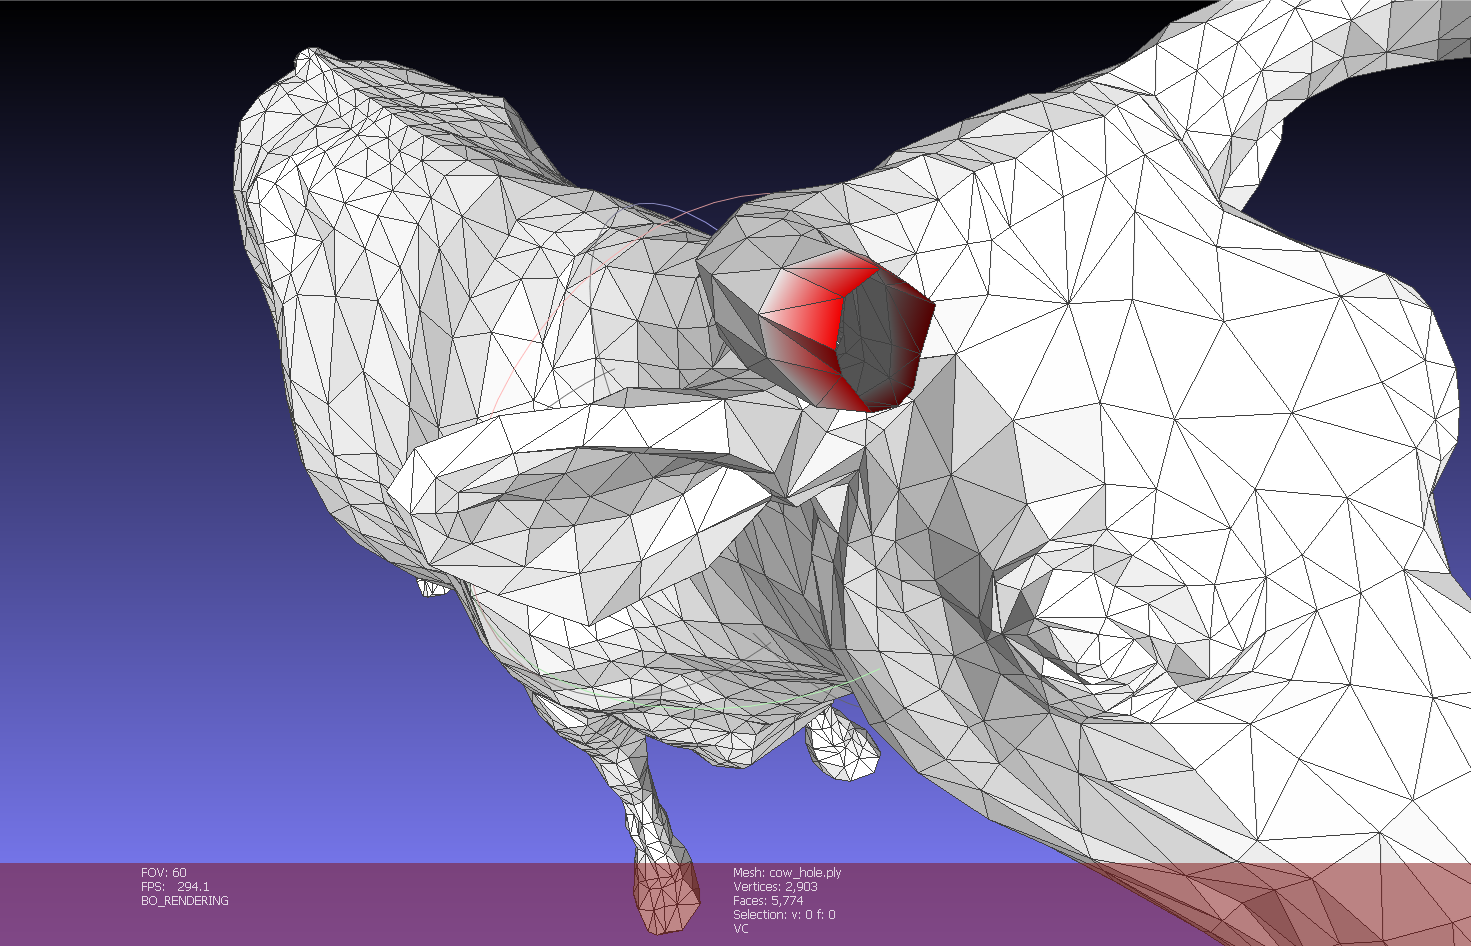
\includegraphics[width=0.45\textwidth]{figures/fig_dataset_cow1.png}
    \hfill
    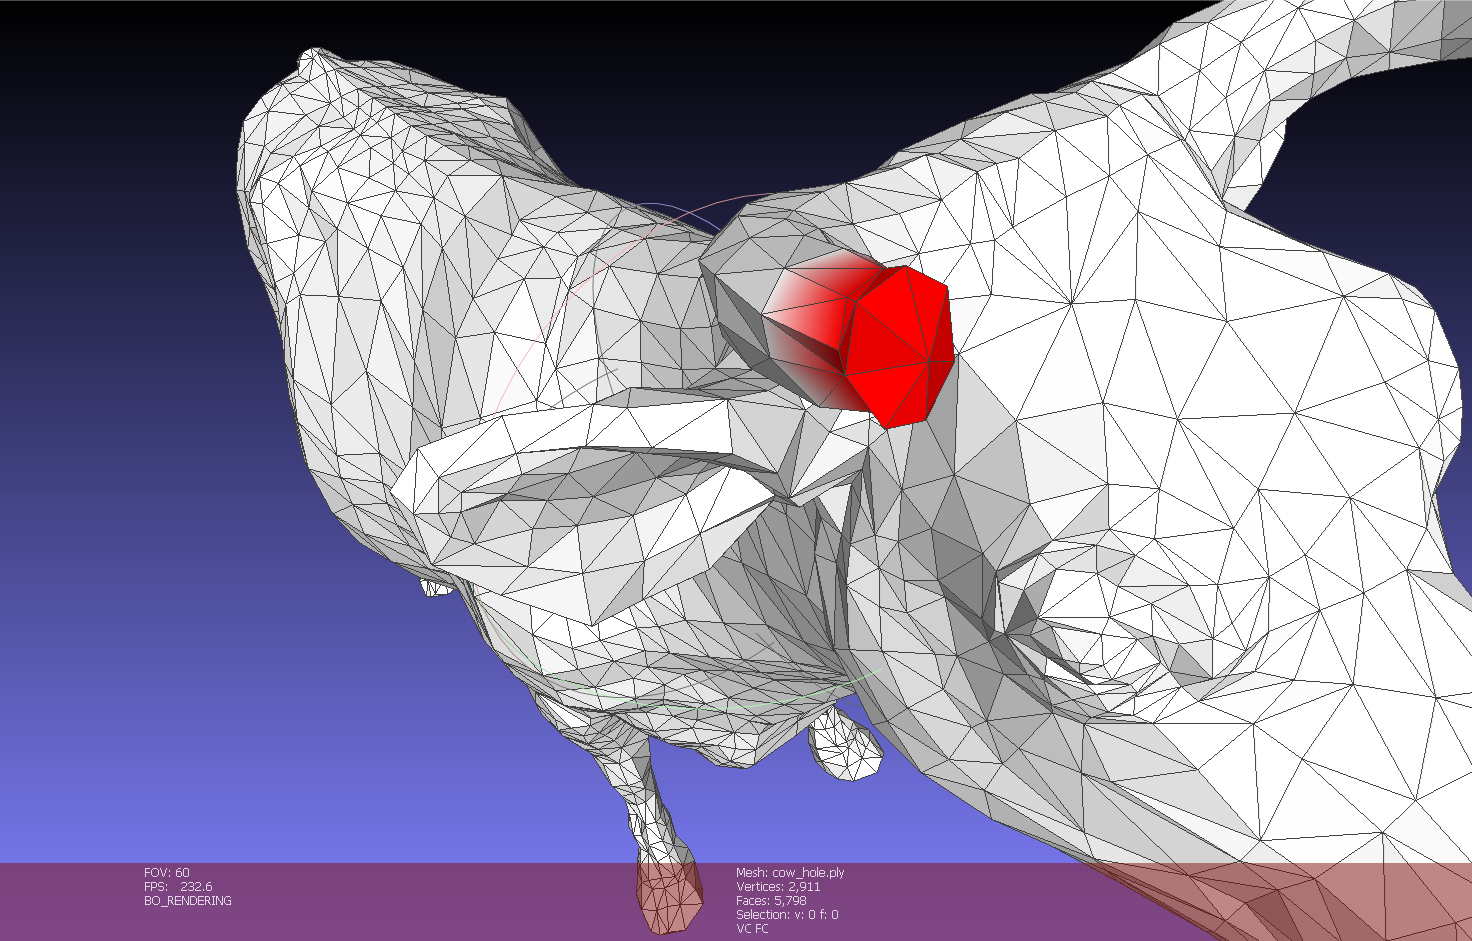
\includegraphics[width=0.45\textwidth]{figures/fig_dataset_cow2.png}
    \caption{\texttt{cow}: input (left) and NFD result (right).}
    \label{fig:dataset-cow}
\end{figure}

\section{Comparison with MeshLab Close Holes}

\begin{figure}[H]
    \centering
    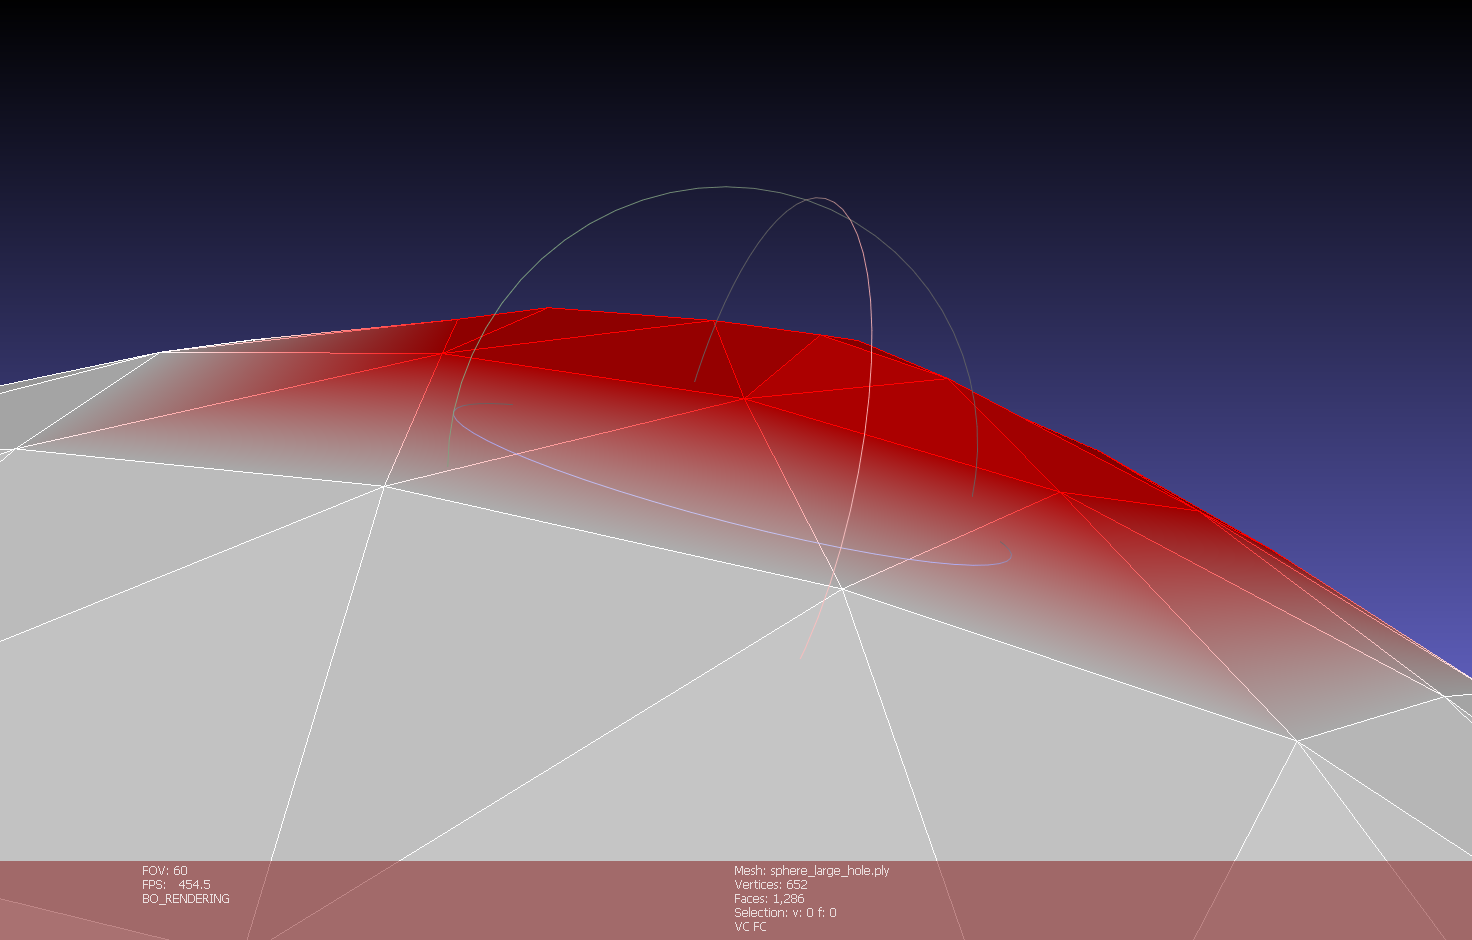
\includegraphics[width=0.45\textwidth]{figures/fig_compare_nfd_closeholes1.png}
    \hfill
    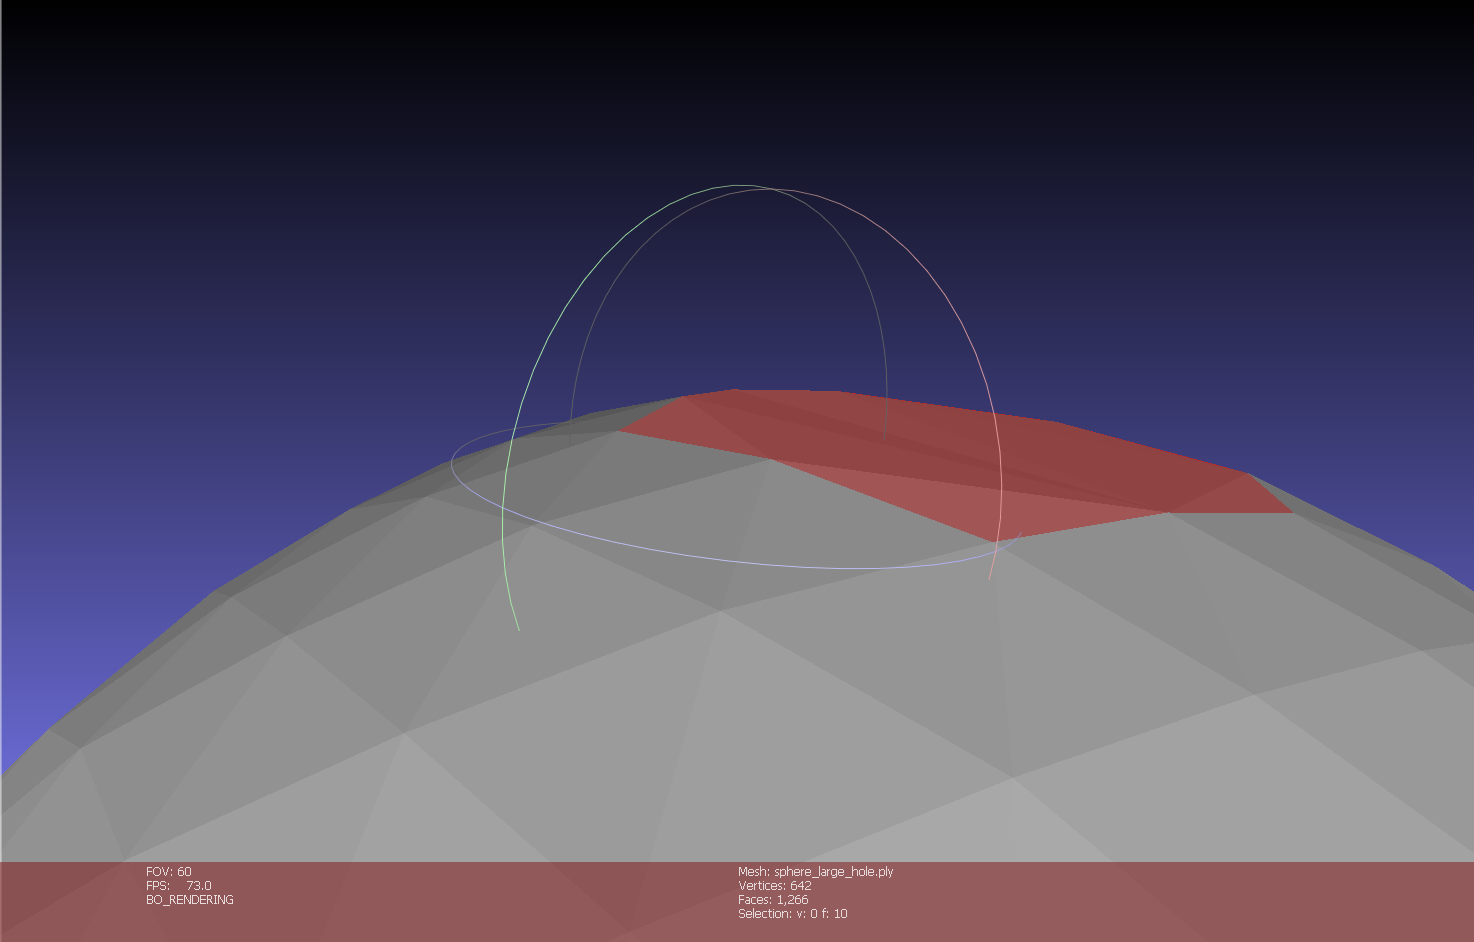
\includegraphics[width=0.45\textwidth]{figures/fig_compare_nfd_closeholes2.png}
    \caption{NFD (left) versus MeshLab \texttt{Close Holes} (right) on the same input.}
    \label{fig:compare-closeholes}
\end{figure}

The visual difference is most pronounced on convex inputs. \texttt{Close Holes} produces a planar triangulation that reads as a flat cap, while NFD bends the patch to follow the surrounding curvature. On a flat region (the side of a cylinder, for instance) the two outputs converge, which is consistent with the model: when $\theta \to 0$ in (\ref{eq:cap-height}), $h \to 0$ and the NFD displacement vanishes.

Figure~\ref{fig:delaunay-compare} shows the effect of the Delaunay-flip pass in Stage~3. Without flipping, slivers from ear clipping are clearly visible near the boundary; with flipping the tessellation becomes regular.

\begin{figure}[H]
    \centering
    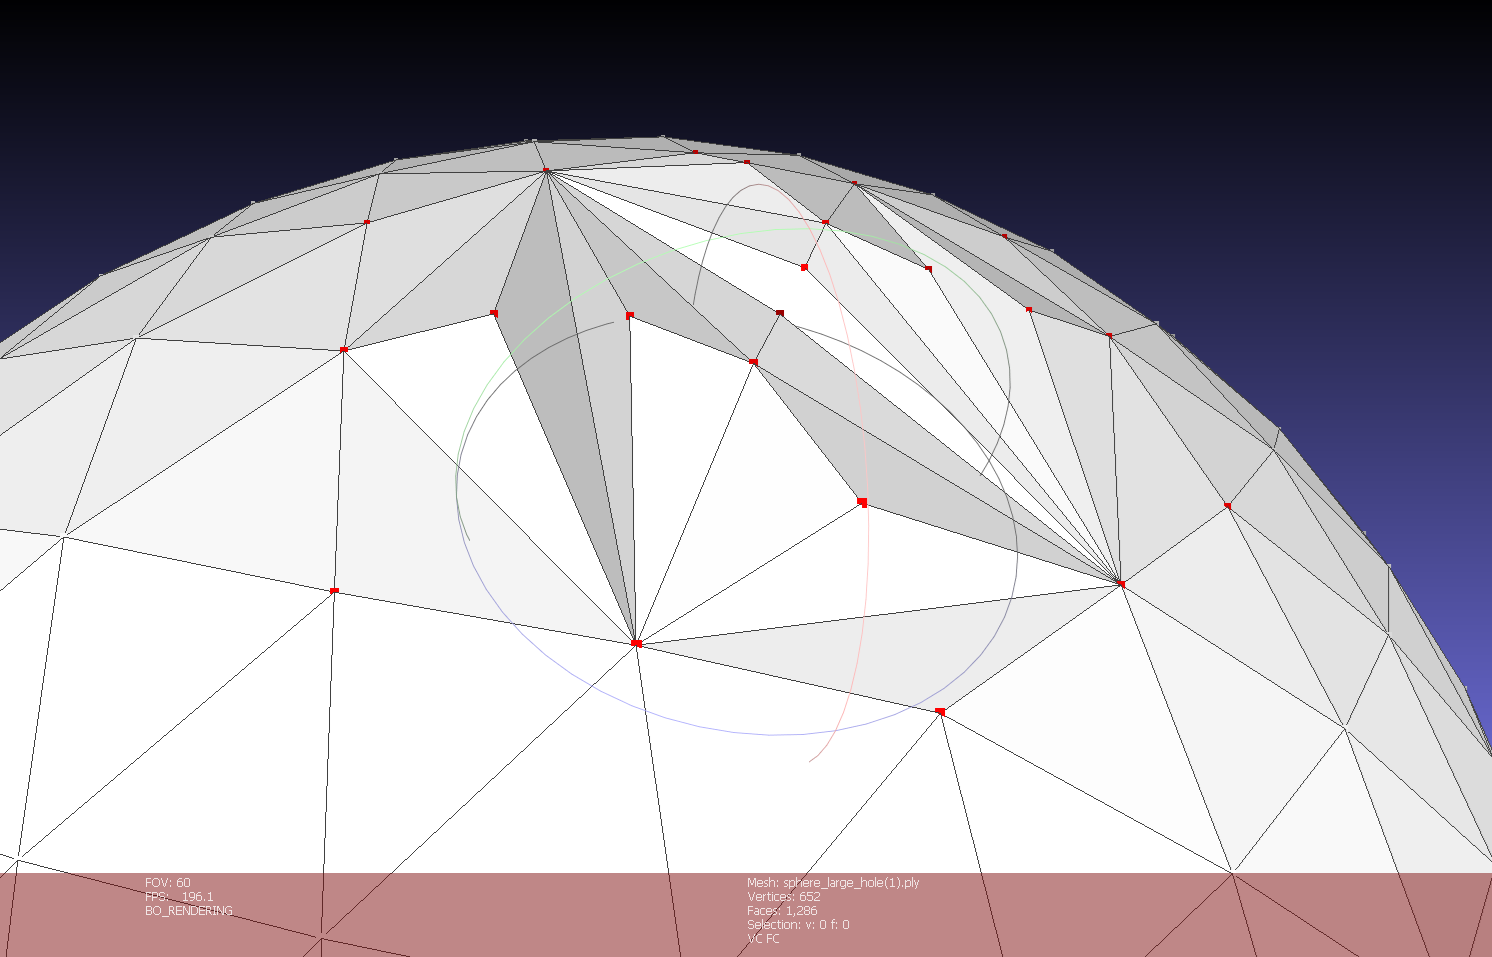
\includegraphics[width=0.45\textwidth]{figures/delaunay_off.png}
    \hfill
    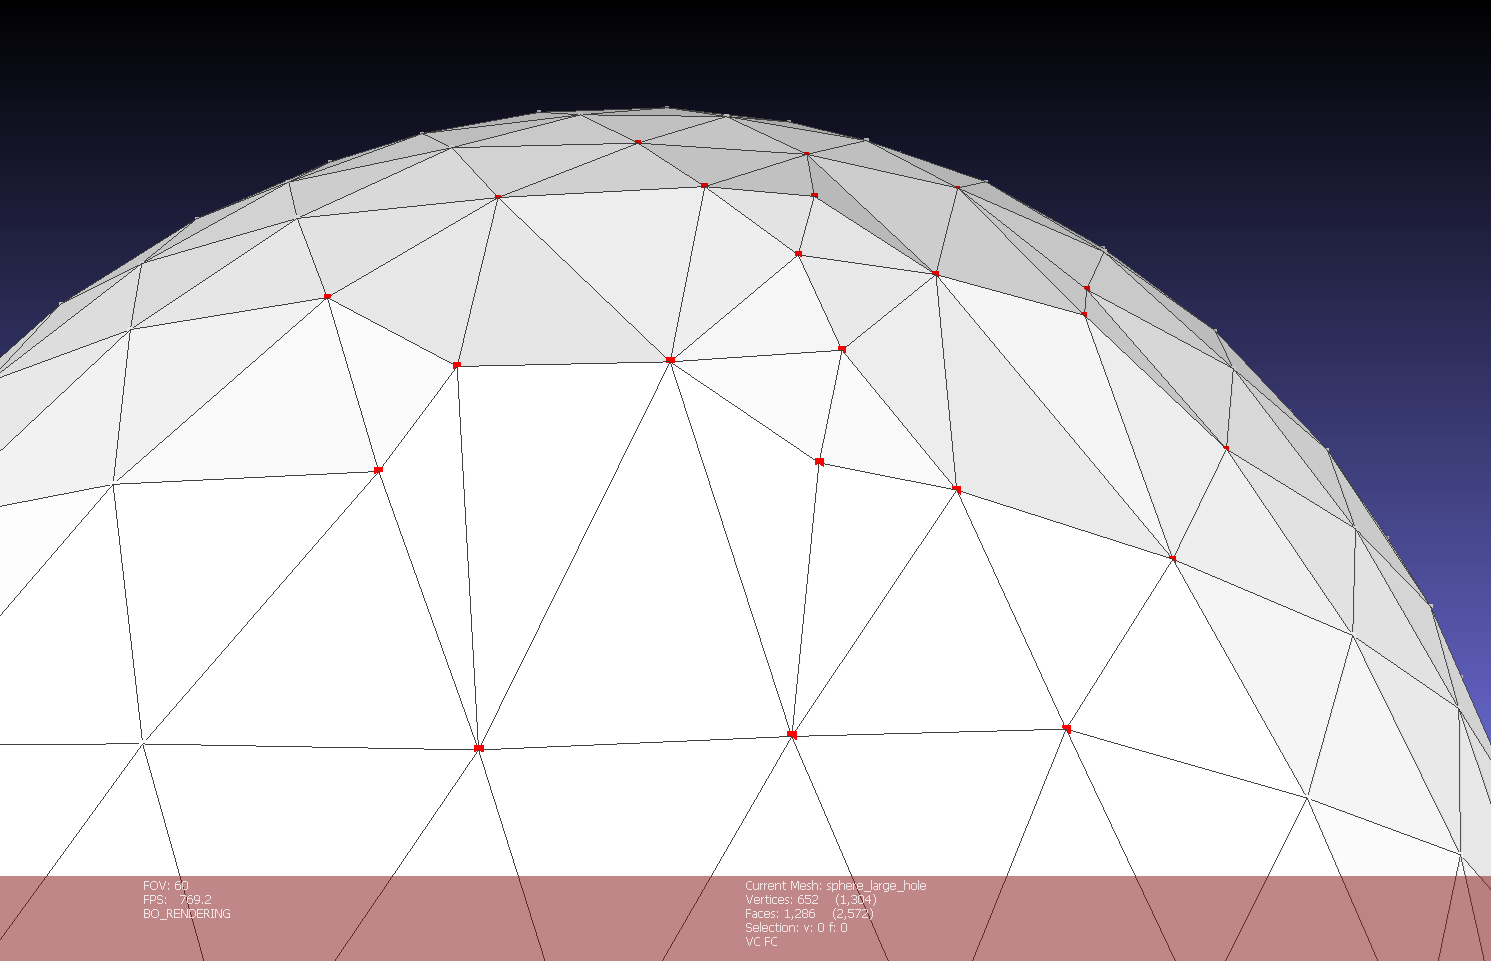
\includegraphics[width=0.45\textwidth]{figures/delaunay_on.png}
    \caption{Ear clipping without (left) and with (right) Delaunay edge flipping.}
    \label{fig:delaunay-compare}
\end{figure}

\section{Performance}

Wall-clock timings on a single thread of an Intel Core i7-12700H, averaged over five runs:

\begin{table}[H]
\centering
\caption{Single-threaded timings.}
\label{tab:timings}
\begin{tabularx}{\textwidth}{l r r X}
\toprule
\textbf{Model} & \textbf{Hole size} & \textbf{Total} & \textbf{Dominant stage} \\
\midrule
\texttt{sphere\_small} & 30 edges & 45 ms  & Stage 3 (triangulation) \\
\texttt{sphere\_large} & 80 edges & 210 ms & Stage 4 (factorisation + solves) \\
\texttt{bunny} (6 holes) & $\sim\!40$ each & 890 ms & sum over six patches \\
\bottomrule
\end{tabularx}
\end{table}

Stage~4 takes 40--60\% of the total on medium holes; the $LDL^T$ factorisation is the single most expensive step but is amortised over 50 solves. Stage~3 takes another 20--30\%, mostly because of the second Delaunay flip pass after centroid refinement. The remaining stages contribute negligibly. All runs complete in well under one second per hole, which is acceptable for interactive use inside MeshLab.

\chapter{DISCUSSION}

\section{Behaviour at default parameters}

Across the test set under default parameters, the symmetric Hausdorff error stays under 1\% of the bounding-box diagonal on the sphere and torus tests, and the per-iteration cost of the diffusion solver remains low because of the one-time Cholesky factorisation. The spherical-cap displacement model produces a usable dome height on inputs that are even approximately spherical without any user tuning, and the $\sqrt{2t-t^2}$ profile gives a patch that meets the surrounding mesh without a visible crease. The plugin runtime fits within MeshLab's interactive loop on every input tested.

\section{Failure modes}

Two failure patterns appeared often enough during testing to be worth describing.

The first is \emph{overshoot}: when boundary normals are noisy or the hole sits in a region of unusually high curvature, the dome height computed from \eqref{eq:cap-height} comes out too large and the patch reads as a raised bump (Figure~\ref{fig:failure-overshoot}). Lowering \texttt{CurvatureStrength} to $0.6$ or $0.7$ corrects most cases. A trimmed mean for $\theta$ would help further but is not implemented in the current version.

\begin{figure}[H]
    \centering
    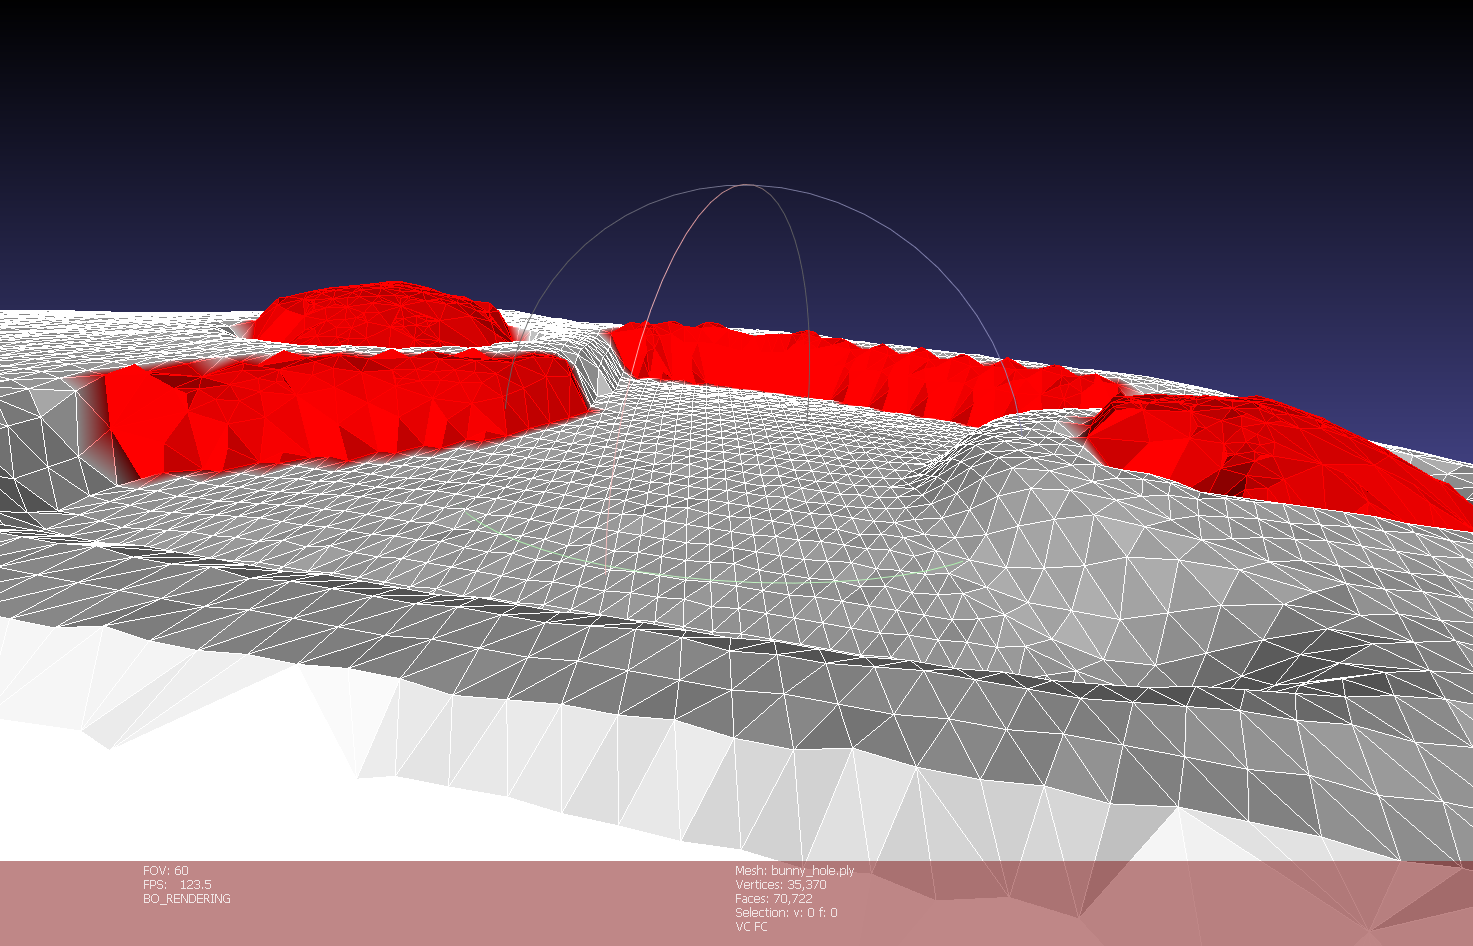
\includegraphics[width=0.55\textwidth]{figures/fig_failure_overshoot.png}
    \caption{Overshoot with \texttt{CurvatureStrength = 1.5} on a sharp Bunny hole.}
    \label{fig:failure-overshoot}
\end{figure}

The second is \emph{under-coverage}: on large holes, with the cow as the worst case, the patch sits on the true surface but does not fully span the removed region, and the reverse-direction Hausdorff distance grows accordingly. Adding interior vertices through smaller \texttt{RefinementFactor} and larger \texttt{DiffusionIterations} reduces the error, but only up to a point: the spherical-cap assumption itself becomes inappropriate for elongated or non-convex hole shapes.

\section{Limitations}

A number of cases lie outside the scope of the current implementation.

The hole detection in Stage~1 walks one boundary loop at a time and assumes a clean 2-manifold input. Holes that share vertices, holes nested inside other holes, and non-manifold edges produce undefined behaviour. In practice, running MeshLab's own non-manifold cleanup before NFD is a workable preprocessing step.

The patch carries vertex colour, averaged from the boundary, but not texture coordinates or material indices. The original Verdera et~al.\ paper extends normal diffusion to texture inpainting, which the present implementation does not.

Sharp features that pass through the hole are not preserved; the patch is uniformly smooth. Recovering them would require detecting crease edges near the boundary and adding them as additional Dirichlet constraints in the diffusion solver, which is more involved than the rest of the pipeline.

The number of diffusion iterations is fixed rather than tolerance-driven. On the test meshes 50 iterations is sufficient, but a residual-based stopping criterion $\|\mathbf{n}^{t+1} - \mathbf{n}^{t}\| < \tau$ would behave more reliably across a wider range of mesh sizes.

\chapter{CONCLUSION}

This report has described a MeshLab plugin that fills holes by diffusing the boundary normal field across the patch interior using the heat equation. After the diffusion converges, interior vertices are displaced along the diffused normals by an amount estimated from the boundary geometry. The output is a patch that follows the surrounding curvature, which classical fillers do not. On the test set, the symmetric Hausdorff error stays sub-percent on sphere-like inputs and is roughly $2$--$4\times$ smaller than MeshLab's built-in \texttt{Close Holes} on curved surfaces.

The mathematical core of the project lies in the combination of standard ingredients: cotangent Laplacian, implicit Euler with a one-time Cholesky factorisation, the spherical-cap height estimate, the $\sqrt{2t-t^2}$ profile, and Taubin smoothing. The ordering of the stages turned out to matter as much as the choice of operators. In particular, applying uniform Laplacian smoothing after the displacement of Stage~6 silently flattens the dome, because uniform smoothing has the shrinkage property that Taubin was designed to avoid.

Looking back, the parts of the project that ate the most time were not the conceptually hardest. Building MeshLab from source and getting the plugin scaffolding (CMake, Qt MOC, plugin discovery, Eigen include paths) lined up correctly took longer than expected; the algorithm is invariant under build-system pain, but a successful first compile is not. The matrix assembly for Stage~4 --- mapping interior vertices to compact indices, accumulating cotangent triplets with the right symmetry, and feeding the result to \texttt{SimplicialLDLT} --- was the second sink, mostly off-by-one indexing rather than anything mathematically deep. Tuning the Taubin coefficients in Stage~6 to balance spike removal against dome preservation came third.

Three extensions seem worth pursuing.
A residual-based stopping criterion in the diffusion loop would replace the fixed iteration count and behave more uniformly across mesh sizes.
A partitioned cap model that fits a separate cap to each ``wedge'' of the boundary would address the saddle-shaped boundaries on which the global cap fit produces visible bias.
Sharp-feature preservation by detecting crease edges near the boundary and adding them as Dirichlet constraints would close the gap with thin-plate methods on inputs that contain creases.


%
\newpage
\chapter*{\begin{center}{\Large \textbf{REFERENCES}}\end{center}}
\addcontentsline{toc}{chapter}{REFERENCES}
\printbibliography[heading=none]

% ---------------- APPENDIX ----------------
\newpage
\CustomChapter{APPENDIX}
\addcontentsline{toc}{chapter}{APPENDIX}

\section*{A. Build environment}

\begin{table}[H]
\centering
\begin{tabularx}{\textwidth}{l X}
\toprule
CPU / RAM & Intel Core i7-12700H / 16 GB DDR5 \\
OS / Compiler & Windows 11 / MSVC 19.41 (VS 2022) \\
Build & CMake 3.28 + Ninja \\
Qt / VCGlib / Eigen & 5.15.2 / MeshLab sub-module / 3.4 \\
Host & MeshLab 2023.12, built from source \\
Eval filter & Filters \textgreater{} Sampling \textgreater{} Hausdorff Distance \\
\bottomrule
\end{tabularx}
\end{table}

\section*{B. Notation}

\begin{table}[H]
\centering
\begin{tabularx}{\textwidth}{l X}
\toprule
$\mathcal{M} = (V, F)$ & Triangle mesh \\
$\partial \Omega$ & Hole / patch boundary \\
$\mathbf{n}_i$ & Unit normal at vertex $v_i$ \\
$L_{\text{cot}}$, $w_{ij}$ & Cotangent Laplacian and edge weights \\
$\alpha_{ij}, \beta_{ij}$ & Angles opposite edge $(v_i, v_j)$ \\
$H_i$ & Mean curvature at $v_i$ \\
$\lambda, \mu$ & Taubin coefficients \\
$r, \theta, h$ & Mean boundary radius, mean angle, cap height \\
$w(t) = \sqrt{2t-t^2}$ & Displacement profile \\
$t_i$ & Normalised geodesic distance from boundary \\
\bottomrule
\end{tabularx}
\end{table}

\end{document}
